\documentclass{tietreport}

% Import images
\usepackage{graphicx}
\usepackage{booktabs}
\usepackage{longtable}
\usepackage{array}
\usepackage{float}
\usepackage{placeins}
\usepackage{rotating}

% Bibliography configuration
\usepackage[
  date=year,
  style=alphabetic,
  backend=biber,
  sorting=nty,
  maxnames=5,
  minnames=3,
  maxalphanames=4,
  minalphanames=3,
  backref=true,
  doi=false,
  isbn=false,
  url=false,
  eprint=false
]{biblatex}
\addbibresource{references.bib}

% Give TeX room to resolve awkward lines containing long
% typewriter identifiers rather than overflowing the margin.
\setlength{\emergencystretch}{3em}
% Keep floats inside the section that refers to them.
\let\oldsection\section
\renewcommand{\section}{\FloatBarrier\oldsection}

%% ==================================================
%% CUSTOMIZE THESE FIELDS FOR YOUR PROJECT
%% ==================================================

% Course/Lab header
\TitlePageHeader{%
  UCS 503 Software Engineering Project Report%
}

% Main project title
\ProjectTitle{%
  CampusCycle%
}

% Subtitle or project description
\ProjectSubTitle{%
  Smart Campus Bicycle Sharing and
  Mobility Management System%
}

% Student information
\author{%
  \texttt{1024030014} Guneet Singh Nagi \\
  \texttt{1024031153} Prabhnoor Oberoi%
}

% Group number, degree, year, program
\TitlePageSubText{%
  Group: \texttt{GROUP-NO} BE Third Year, CSE%
}

% Faculty advisor/guide name
\AdvisorName{%
  ADVISOR-NAME%
}

% Evaluation period and department info
\TitlePageFooterText{{%
    \large End-Semester Evaluation \\[0.2cm]
    \bfseries Computer Science and Engineering
    Department%
  } \\[0.15cm]
  Thapar Institute of Engineering and Technology,
  Patiala%
}

%% ==================================================

\begin{document}

% Generate title page
\maketitle

% Table of contents (auto-generated from chapters)
\tableofcontents

% ===== CHAPTER 1: INTRODUCTION =====

\chapter{Introduction}

\section{Background and Context}

A university campus is large enough that walking
between a hostel, an academic block, the library and
the sports complex consumes a noticeable part of a
student's day, yet far too small for motorised
transport to be worthwhile. This is the classic
last-mile problem, and shared bicycles are a
well-established answer to it: public bike-sharing
schemes have been deployed in several hundred cities
worldwide, and the research literature consistently
identifies availability information and fleet
maintenance as the factors that decide whether such a
scheme is used or abandoned~\cite{shaheen2010,
fishman2016}. Both are information problems rather
than hardware problems, which is what makes a campus
scheme a suitable software engineering project.

A bicycle-sharing scheme is not solved by buying
bicycles. Without a system behind them, the fleet
accumulates the familiar failures: cycles pile up at
one stop while another stands empty, a bicycle with
failed brakes is rented out because nobody recorded
the fault, cycles leave the campus and are not
recovered, and the administration has no evidence on
which to base decisions about where cycles should be
placed.

CampusCycle addresses that gap. It is a web
application through which a student finds an available
bicycle on a map of the campus, plans a route to it
along the roads that actually exist, identifies the
cycle by scanning the QR code printed on it, rides
between stops and returns it, while an administrator
manages the fleet, tracks every ride, processes
reported faults and reads usage analytics computed
from the live database.

\subsection{Problem Statement}

Design and build a centralised system for managing a
campus bicycle-sharing service that:

\begin{enumerate}
  \item tells a student, accurately and in real time,
    where a usable bicycle can be found, and how to
    get between two stops on the campus road network;
  \item records every rental from start to finish so
    that a cycle is never in two places at once and a
    student never holds two cycles at once;
  \item ensures that a bicycle reported as unsafe
    cannot be rented out again until it has been
    inspected; and
  \item gives the administration figures about fleet
    utilisation, stop demand and maintenance load that
    are computed from the system's own records rather
    than estimated.
\end{enumerate}

The difficulty in such a system is not any single
feature. It is that several of these requirements are
\emph{invariants} rather than screens: statements that
must hold no matter which part of the application is
running, and no matter how many users act at the same
time. Much of the design work reported here is
concerned with where such invariants are enforced, and
the data-flow diagrams in Chapter~2 are annotated to
show exactly which flows carry them.

\section{Project Objectives}

The objectives below were set in the project proposal.
Each is stated with the criterion by which it is
judged, and its status at this final evaluation.

\begin{enumerate}
  \item \textbf{Account management and role
    separation.} Students register and sign in; an
    administrator console is reachable only by an
    administrator account. \emph{Criterion:} every
    administrative endpoint rejects a student token.
    \emph{Status: complete.}

  \item \textbf{QR-based bicycle identification.} Each
    bicycle carries a unique QR code which the backend
    resolves to a bicycle record and its current
    state. \emph{Criterion:} an unknown code and an
    unavailable cycle are both refused, with distinct
    responses. \emph{Status: complete.}

  \item \textbf{Rental and return workflow.} A student
    starts a ride, sees it in progress and returns the
    cycle at an approved stop. \emph{Criterion:} two
    students attempting the same cycle at the same
    instant produce exactly one rental.
    \emph{Status: complete.}

  \item \textbf{Interactive campus map.} Stops are
    shown on a map of the campus with their live
    availability. \emph{Criterion:} the map and the
    stop list never disagree, because both derive
    availability from one rule.
    \emph{Status: complete, and extended in Phase~3
    to the illustrated campus map with road-following
    route planning (Section~\ref{sec:map}).}

  \item \textbf{Complete rental records.} Every ride
    is retained and can be inspected by the student
    who took it and by an administrator.
    \emph{Criterion:} a student cannot read another
    student's ride, by any route.
    \emph{Status: complete.}

  \item \textbf{Fault reporting and maintenance
    management.} Students report faults; the
    administration works them through a defined
    lifecycle. \emph{Criterion:} a cycle with an
    unresolved safety fault cannot be rented or
    returned to service. \emph{Status: complete.}

  \item \textbf{Usage analytics.} The administration
    sees fleet, stop and ridership figures over a
    selectable period. \emph{Criterion:} every figure
    is a database aggregate, and the page survives an
    empty database. \emph{Status: complete.}

  \item \textbf{Campus geofencing.} A configurable
    campus boundary, with violations recorded and
    surfaced for action. \emph{Criterion:} a repeated
    breach does not produce repeated alerts.
    \emph{Status: complete as a software
    demonstration; see Section~\ref{sec:geofence}
    for the limitation that matters.}

  \item \textbf{Demand prediction and redistribution.}
    Prediction of stop-level demand from historical
    rentals, and redistribution advice derived from
    it. \emph{Status: not implemented}, for the reason
    given in Section~\ref{sec:scope}. It is carried
    forward as the first item of future work.
\end{enumerate}

Eight of the nine objectives are delivered and
evidenced by the automated tests reported in
Chapter~3. The ninth is stated here as unmet rather
than described in terms that would suggest otherwise.

\section{Scope of This Report}
\label{sec:scope}

Development was organised into three phases, each
ending with a working, tested application.

\begin{itemize}
  \item \textbf{Phase~1 --- the core rental system:}
    accounts and roles, stops, the fleet, QR
    identification, the rental and return workflow,
    and an administrative dashboard.
  \item \textbf{Phase~2 --- information and safety:}
    stop availability, ride history, maintenance
    management with a safety hold, usage analytics and
    software geofencing.
  \item \textbf{Phase~3 --- the campus map:} the
    illustrated campus map with live markers, a
    hand-traced road network, and shortest-path route
    planning between stops.
\end{itemize}

This report covers all three phases. The
machine-learning demand-prediction module was
deliberately held back rather than attempted
alongside them. A demand model is only as good as the
ridership history it is trained on, and that history
is produced by the very modules Phases~2 and~3
deliver; the system has been in demonstration use
rather than campus-wide service, so the recorded
history is seed data and a handful of real rides, not
a term's worth of ridership. Training a model on that
would produce a convincing-looking artefact with no
predictive content. The analytics layer that such a
model would consume is complete and is described in
Section~\ref{sec:analytics}; the model itself is
specified as future work in
Section~\ref{sec:futurework}.

% ===== CHAPTER 2: METHODOLOGY & DESIGN =====

\chapter{Methodology and Design}

\section{Development Approach}

The system was developed incrementally. Each phase was
implemented against the running output of the previous
one under three self-imposed constraints: the existing
database was to be migrated rather than rebuilt, the
existing architectural conventions were to be reused
rather than replaced, and the existing test suites were
to keep passing unchanged. The last of these functioned
as a regression gate; the schema constraint is why all
later schema changes are additive and idempotent
(Section~\ref{sec:migrations}).

Work was tracked in a single Git repository with the
application and all three written deliverables --- the
proposal, the prototype report and this report ---
kept side by side, so that a claim in a report and the
code it describes move together.

\section{System Architecture}

\subsection{High-Level Design}

CampusCycle follows a three-tier architecture
(Figure~\ref{fig:arch}). The browser holds the entire
user interface; the Node.js process holds all business
rules; PostgreSQL holds all state. The two tiers
communicate only over a JSON REST API, which means the
server never produces markup and the browser never
issues a query.

\begin{figure}[htbp]
  \centering
  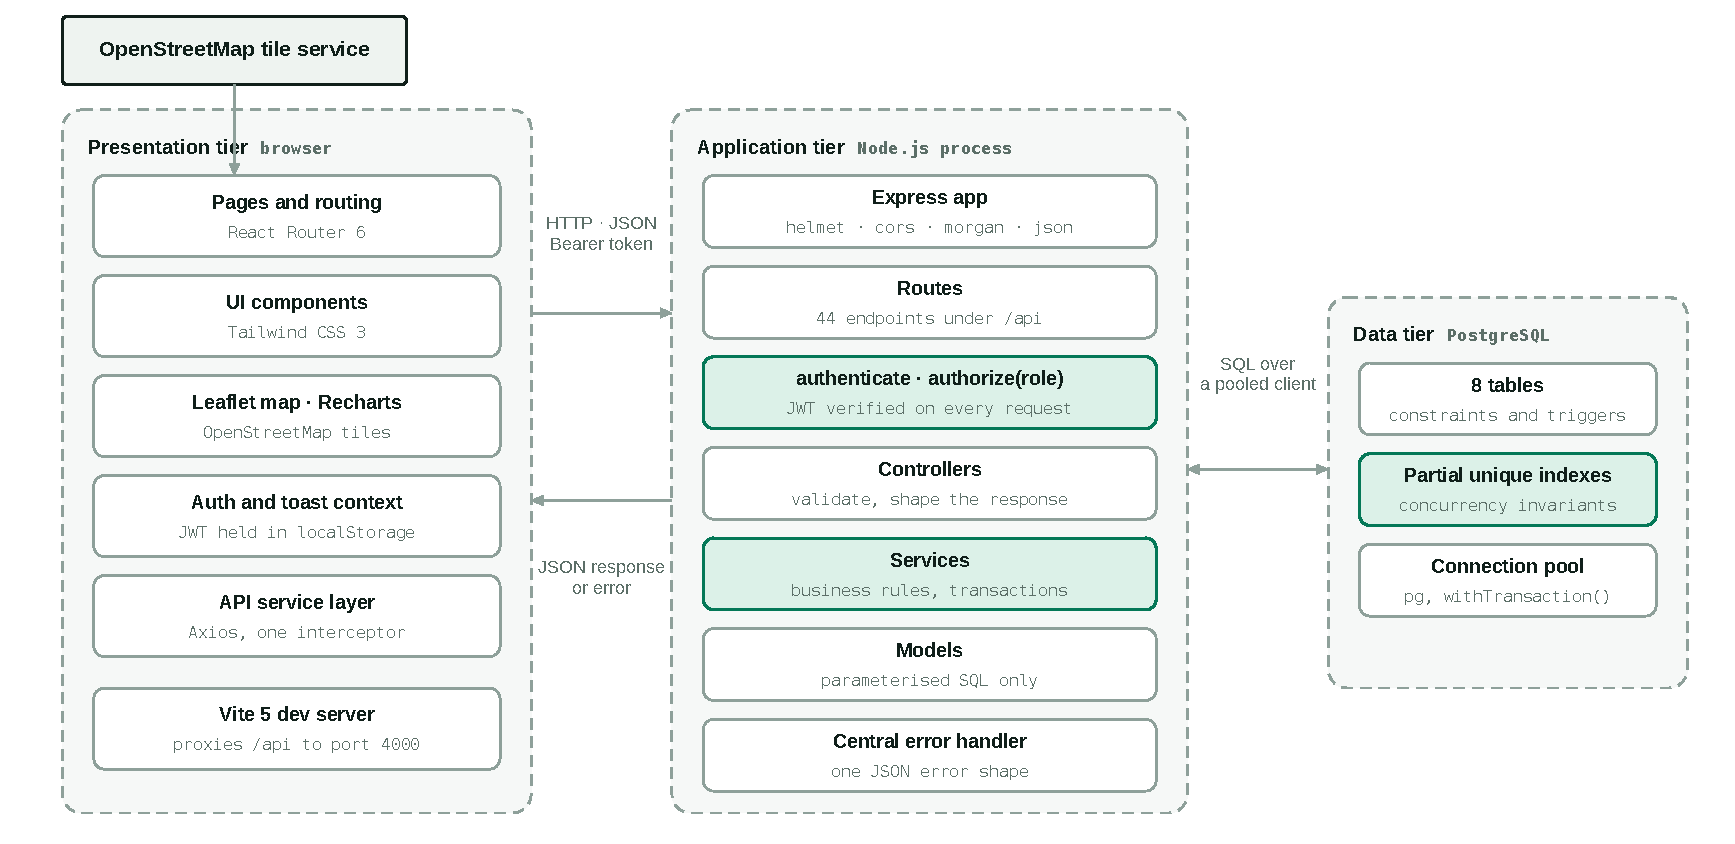
\includegraphics[width=\textwidth]{figures/arch.pdf}
  \caption{Three-tier architecture. Each request
    crosses the server layers in order, and only the
    model layer issues SQL.}
  \label{fig:arch}
\end{figure}

The application tier is deliberately layered, and a
request always crosses the layers in the same order:

\begin{itemize}
  \item \textbf{Routes} declare the URL, the HTTP verb
    and the roles permitted to reach the handler.
  \item \textbf{Middleware} verifies the JSON Web
    Token~\cite{rfc7519} and attaches the caller's
    identity and role to the request.
  \item \textbf{Controllers} read and validate request
    parameters and shape the response. They contain no
    business rules.
  \item \textbf{Services} hold the business rules, and
    own every database transaction.
  \item \textbf{Models} issue parameterised SQL and
    nothing else.
\end{itemize}

Keeping transactions in the service layer, rather than
in controllers or models, is what makes the
concurrency rules in Section~\ref{sec:concurrency}
expressible at all: a rule that spans two tables has
exactly one place it can live.

\subsection{Technical Stack}

\begin{table}[htbp]
\centering
\begin{tabular}{@{}lll@{}}
\toprule
\textbf{Layer} & \textbf{Technology} &
\textbf{Version} \\
\midrule
User interface   & React with Vite        & 18.3 / 5.4 \\
Styling          & Tailwind CSS           & 3.4 \\
Routing          & React Router           & 6.24 \\
HTTP client      & Axios                  & 1.7 \\
Map rendering    & Leaflet (CRS.Simple)   & 1.9.4 \\
Charts           & Recharts               & 2.15 \\
QR decoding      & jsQR                   & 1.4 \\
Server runtime   & Node.js                & $\geq 18$ \\
Web framework    & Express                & 4.19 \\
Database         & PostgreSQL             & $\geq 13$ \\
Database driver  & node-postgres (pg)     & 8.12 \\
Authentication   & jsonwebtoken, bcryptjs & 9.0 / 2.4 \\
HTTP hardening   & helmet, cors           & 7.1 / 2.8 \\
Version control  & Git and GitHub         & --- \\
\bottomrule
\end{tabular}
\caption{Implementation stack.}
\label{tab:stack}
\end{table}

\subsubsection*{Departure from the proposal:
PostgreSQL in place of MySQL}

The proposal named MySQL. The implementation uses
PostgreSQL, and the reason is specific rather than a
matter of preference. Three of the system's invariants
are enforced by \emph{partial unique
indexes}~\cite{pgindexes} --- unique indexes that
apply only to the rows matching a predicate:

\begin{itemize}
  \item at most one \texttt{ACTIVE} rental per
    student;
  \item at most one \texttt{ACTIVE} rental per
    bicycle;
  \item at most one unresolved geofence alert per
    bicycle.
\end{itemize}

MySQL has no partial indexes, so each of these rules
would have to be enforced in application code, where
it is subject to the race conditions discussed in
Section~\ref{sec:concurrency}. PostgreSQL also
supplies three features the analytics module relies
on: \texttt{FILTER} clauses on aggregates,
\texttt{generate\_series} for producing a continuous
date axis including days on which nothing happened,
and \texttt{JSONB} for storing the geofence polygon.
The cost of the change was confined to the schema
files and the database driver; no application logic
depends on the vendor.

\subsubsection*{Departure from the prototype:
the illustrated campus map}

The prototype rendered stops as markers on
OpenStreetMap tiles. That was replaced in Phase~3 by
an illustrated map of the campus. The reason is
described in Section~\ref{sec:map}; the consequence
for the stack is that Leaflet~\cite{leaflet} is still
used, but in its non-geographic \texttt{CRS.Simple}
mode with the illustration as the only layer. No map
tiles are fetched at run time, and the application no
longer depends on an external tile service.

\section{Data Flow}

The data-flow diagrams use Gane--Sarson
notation~\cite{demarco1979}: an external entity is a
square box, a process is a rounded box carrying a
number band, and a data store is an open-ended box
with its D-number in the left cell. Throughout the
set, a flow drawn in green is one that carries or
enforces a system invariant --- the notation is used
to distinguish rules from traffic.

Figure~\ref{fig:dfd0} fixes the system boundary.
Figure~\ref{fig:dfd1} decomposes the system into nine
processes around the nine stores they use. The five
remaining figures explode the processes whose internal
behaviour is not obvious from the level-1 view:
rentals (Figure~\ref{fig:dfd2r}), maintenance
(Figure~\ref{fig:dfd2m}), geofencing
(Figure~\ref{fig:dfd2g}), analytics
(Figure~\ref{fig:dfd2a}) and route planning
(Figure~\ref{fig:dfd2p}).

\begin{figure}[htbp]
  \centering
  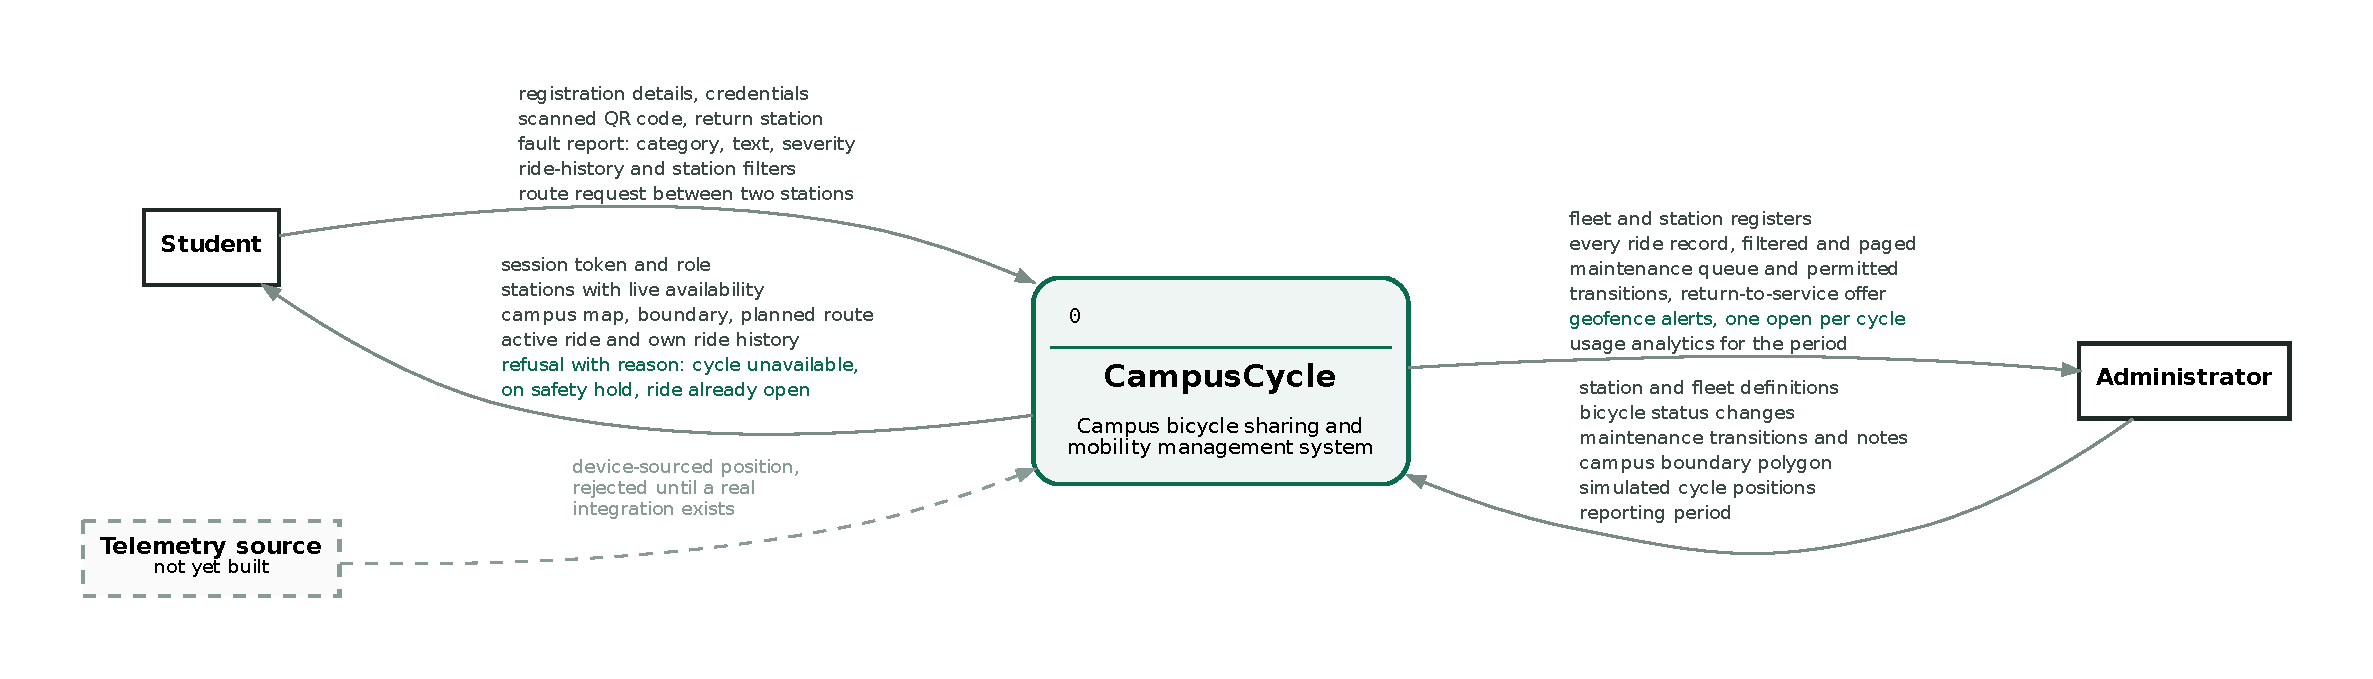
\includegraphics[width=\textwidth]{figures/dfd-l0.pdf}
  \caption{Context diagram. Each arrow is itemised
    rather than summarised, so that the boundary can
    be checked flow by flow. The dashed entity records
    an honest gap: the bicycles carry no telemetry
    hardware, so positions claiming to come from a
    device are refused until a real integration
    exists.}
  \label{fig:dfd0}
\end{figure}

% Turned sideways on a page of its own: at portrait
% width the process labels would be too small to read
% in print.
\begin{figure}[p]
  \centering
  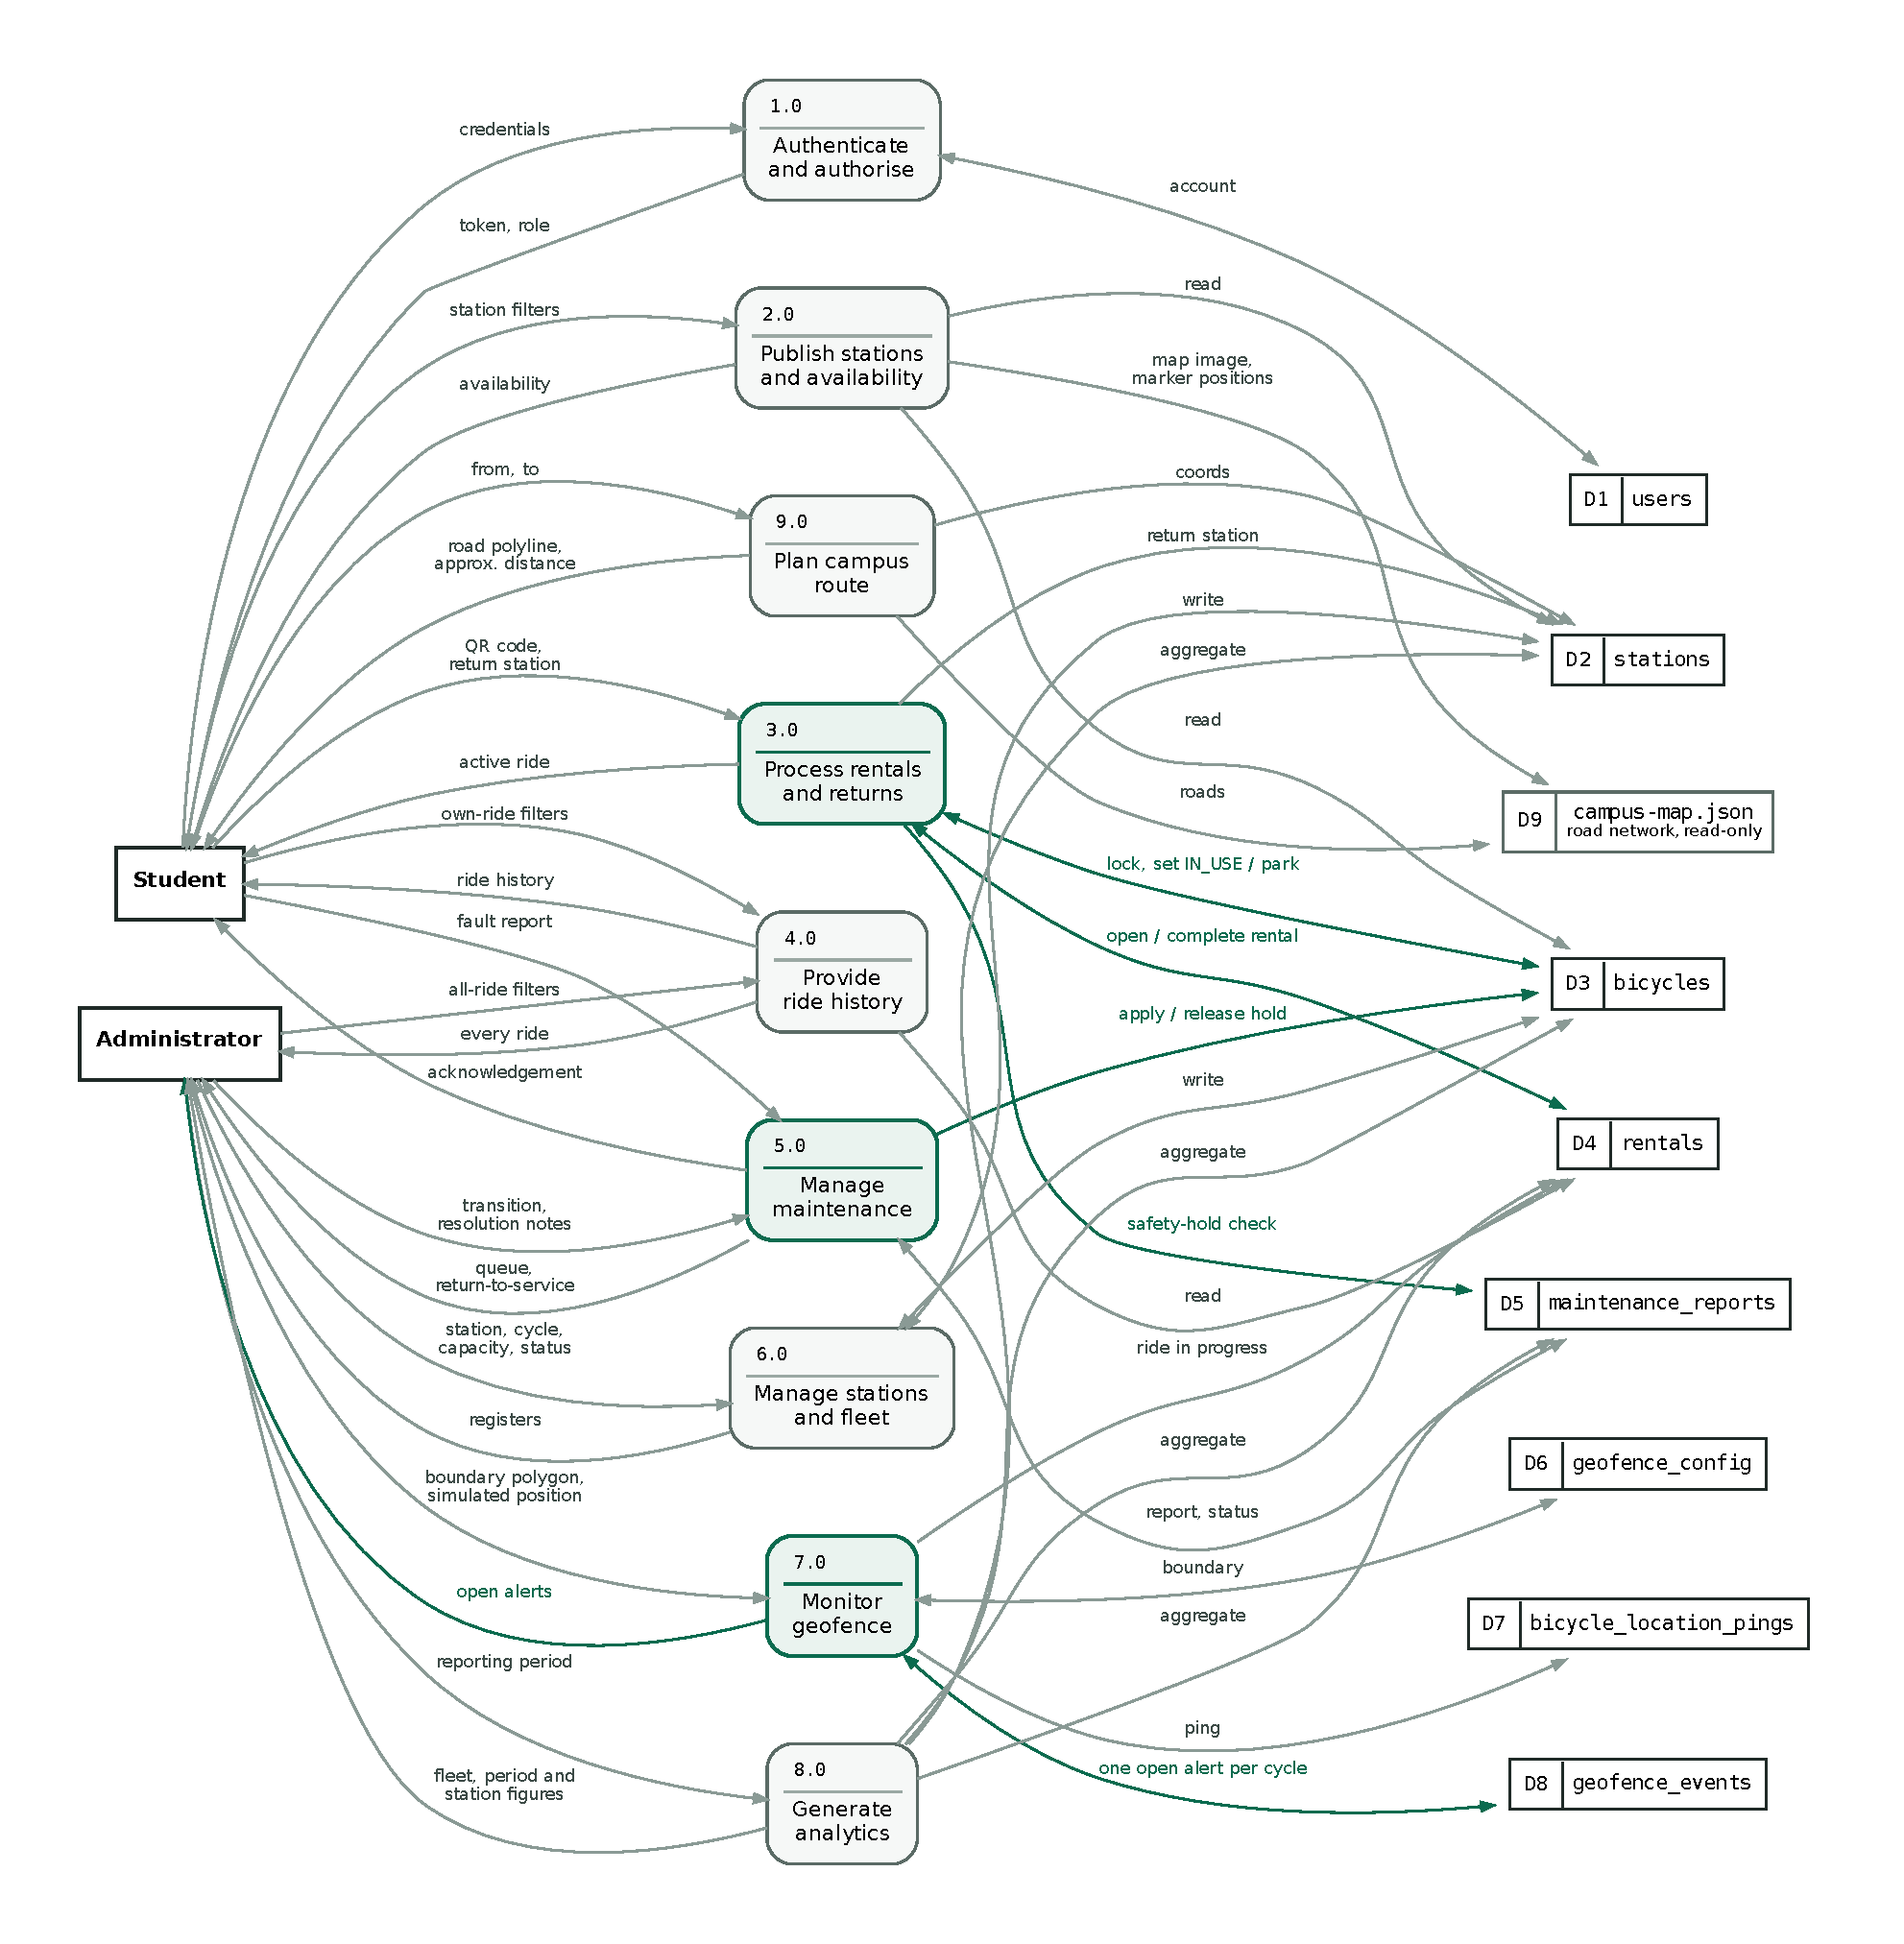
\includegraphics[width=\textwidth]{figures/dfd-l1.pdf}
  \caption{Level-1 data flow diagram. Nine processes
    around the nine stores they use. Writes to a store
    belong to exactly one process; reads cross freely.
    \texttt{D9} is a read-only configuration file, not
    a table.}
  \label{fig:dfd1}
\end{figure}

\subsection{Level 2: Rentals and Returns}

Figure~\ref{fig:dfd2r} explodes process~3.0. It is the
busiest diagram in the set because the rental path is
where four separate rules meet: the rider must hold no
open ride, the cycle must be available, the cycle must
carry no safety hold, and the whole sequence must be
safe against a second request arriving in the middle
of it. Processes 3.2, 3.3 and 3.4 are the three checks;
3.8 is the one that is easy to forget, because a fault
filed while a ride is in progress must take effect when
that ride ends rather than at the moment it is filed.

\begin{sidewaysfigure}
  \centering
  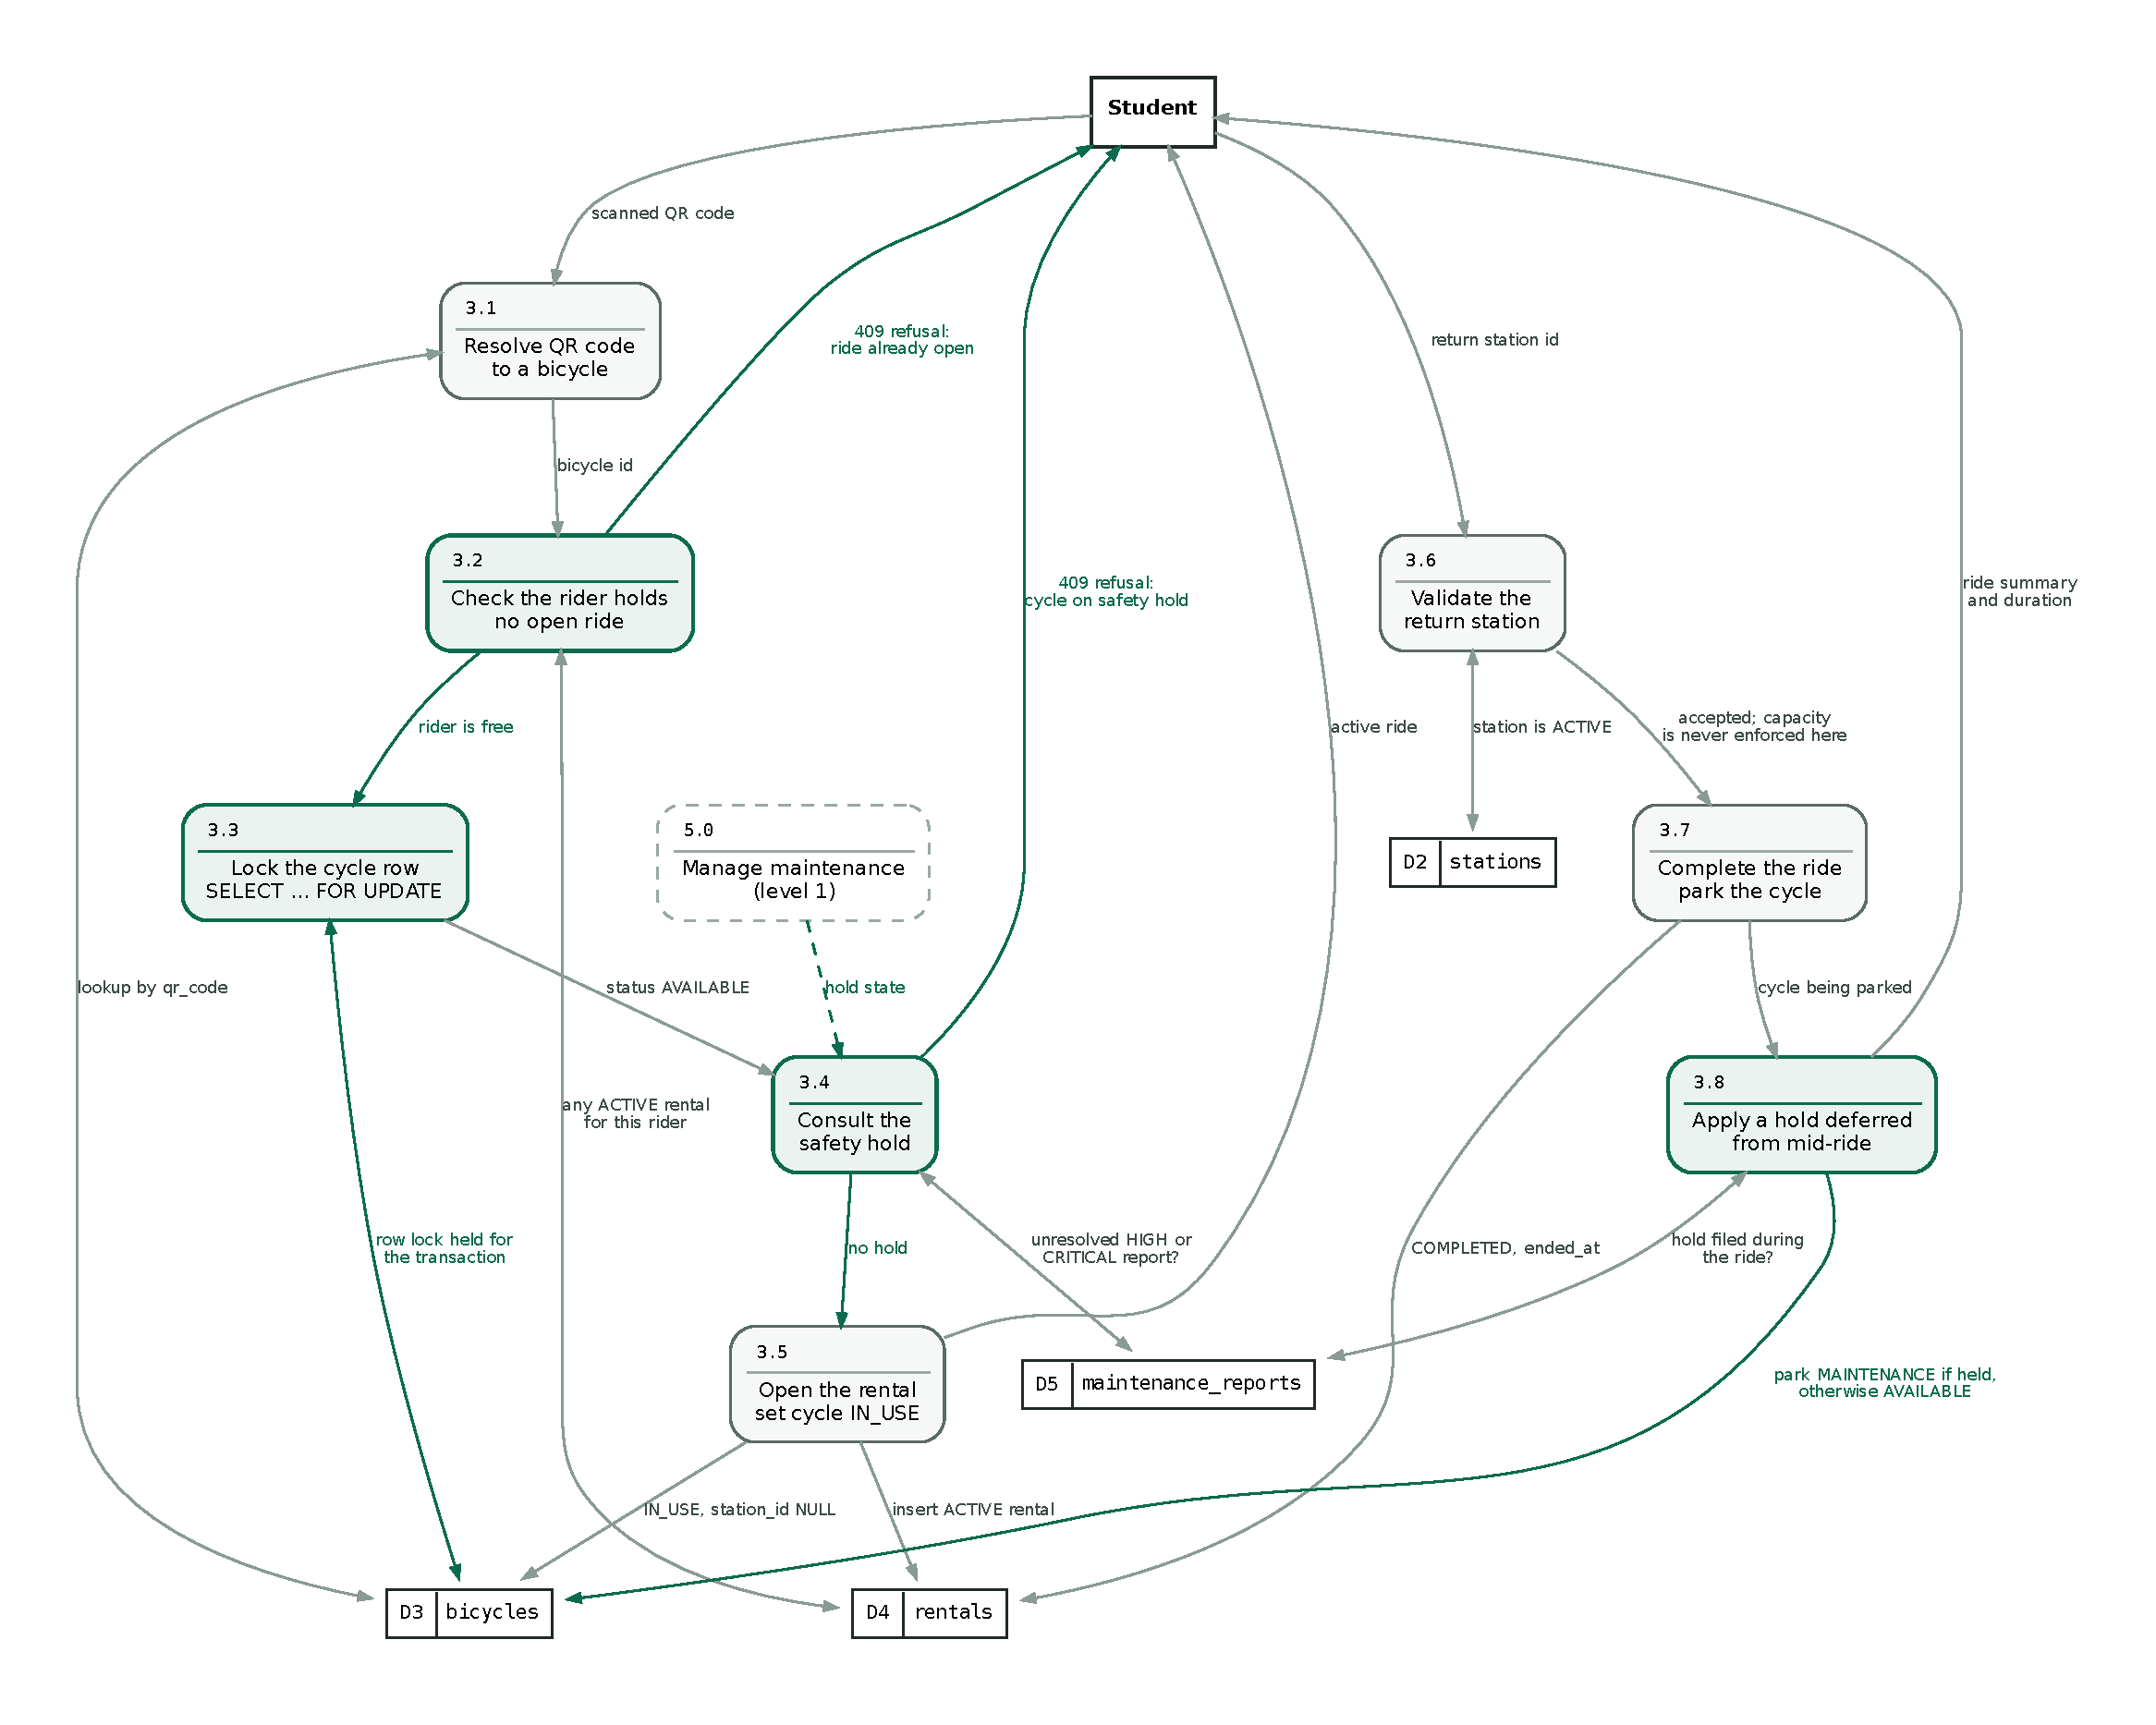
\includegraphics[width=\textheight,height=\textwidth,keepaspectratio]{figures/dfd-l2-rental.pdf}
  \caption{Level-2 diagram for process 3.0, rentals and
    returns. The green path is the invariant: a rental
    is created only after three checks pass inside one
    transaction that holds a row lock on the bicycle.}
  \label{fig:dfd2r}
\end{sidewaysfigure}

\subsection{Level 2: Maintenance and the Safety Hold}

Figure~\ref{fig:dfd2m} explodes process~5.0. This is
the one module where a user-facing feature and a
safety property meet, and the diagram separates the
two routes by which a cycle leaves service --- taken
out immediately when it is parked (5.4), or held until
the current ride ends (5.5) --- from the single route
by which it returns (5.8).

\begin{figure}[p]
  \centering
  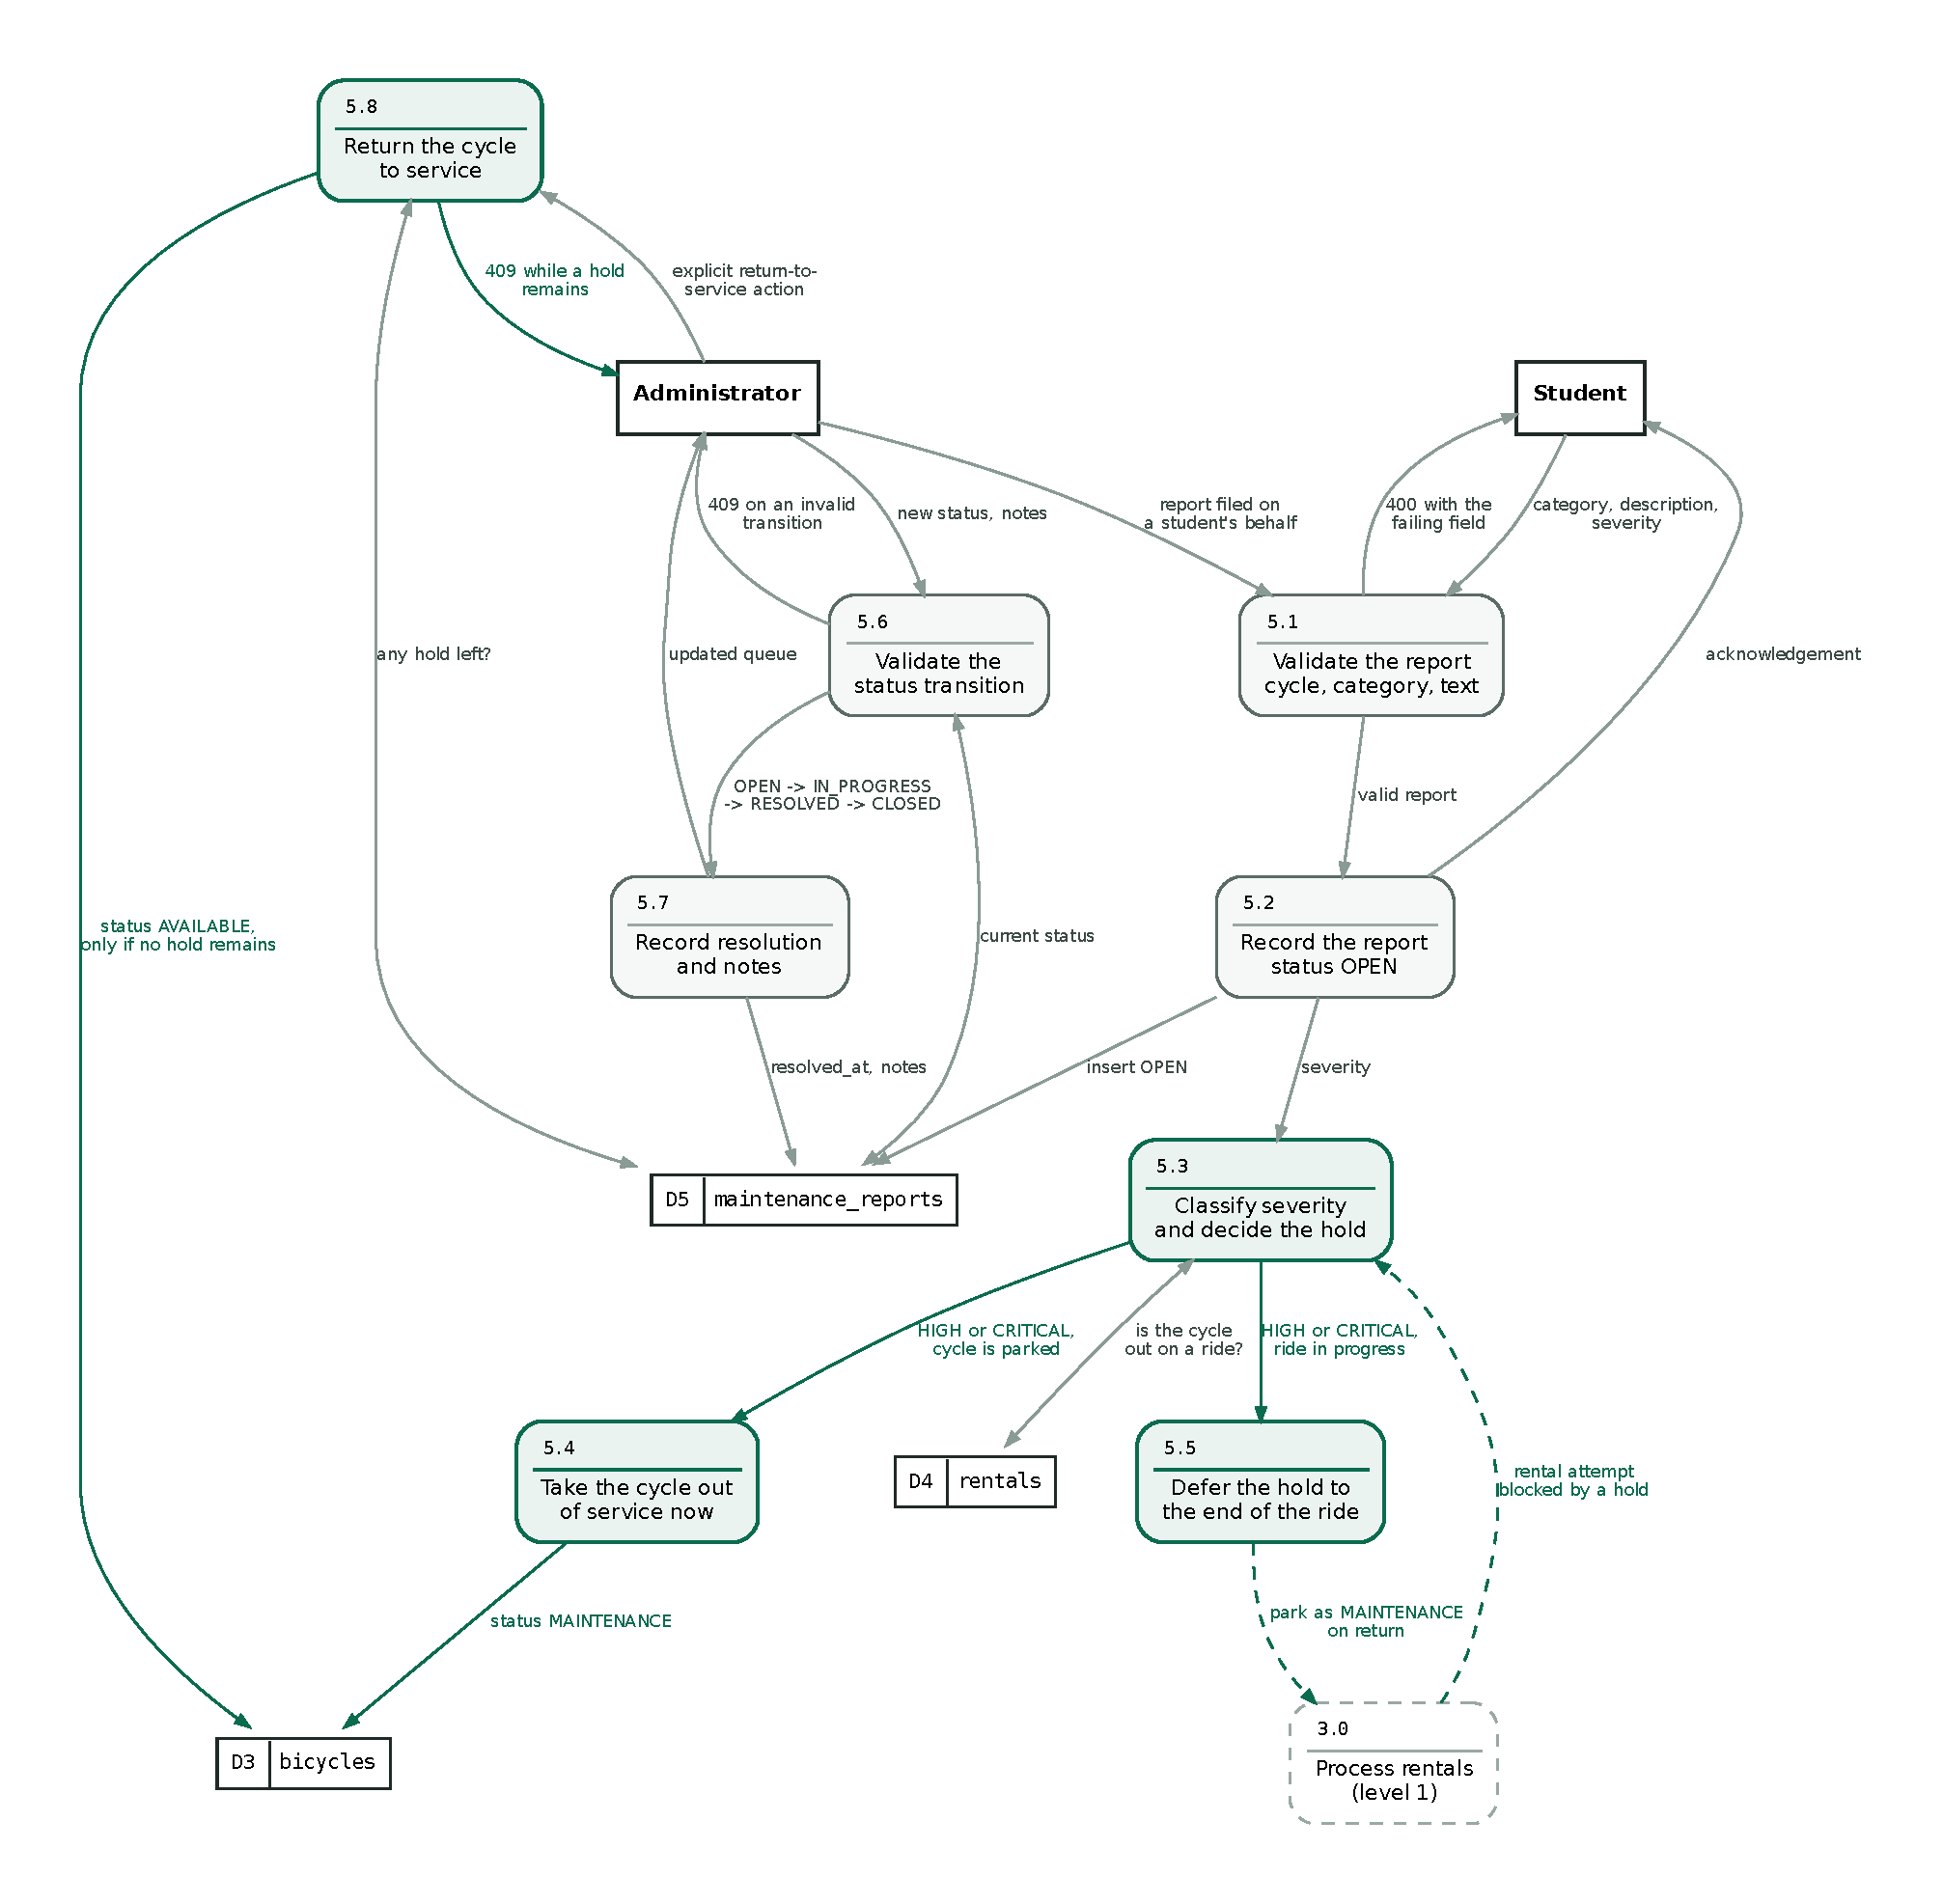
\includegraphics[width=\textwidth]{figures/dfd-l2-maintenance.pdf}
  \caption{Level-2 diagram for process 5.0,
    maintenance. Resolving a report and returning a
    cycle to service are deliberately separate
    processes; 5.8 refuses while any hold remains.}
  \label{fig:dfd2m}
\end{figure}

\subsection{Level 2: Geofencing}

Figure~\ref{fig:dfd2g} explodes process~7.0. The
ordering matters: the caller is authorised (7.1) and
the provenance of the position is validated (7.2)
before anything is stored, so no unvalidated position
ever reaches the store or the boundary test.

\begin{figure}[p]
  \centering
  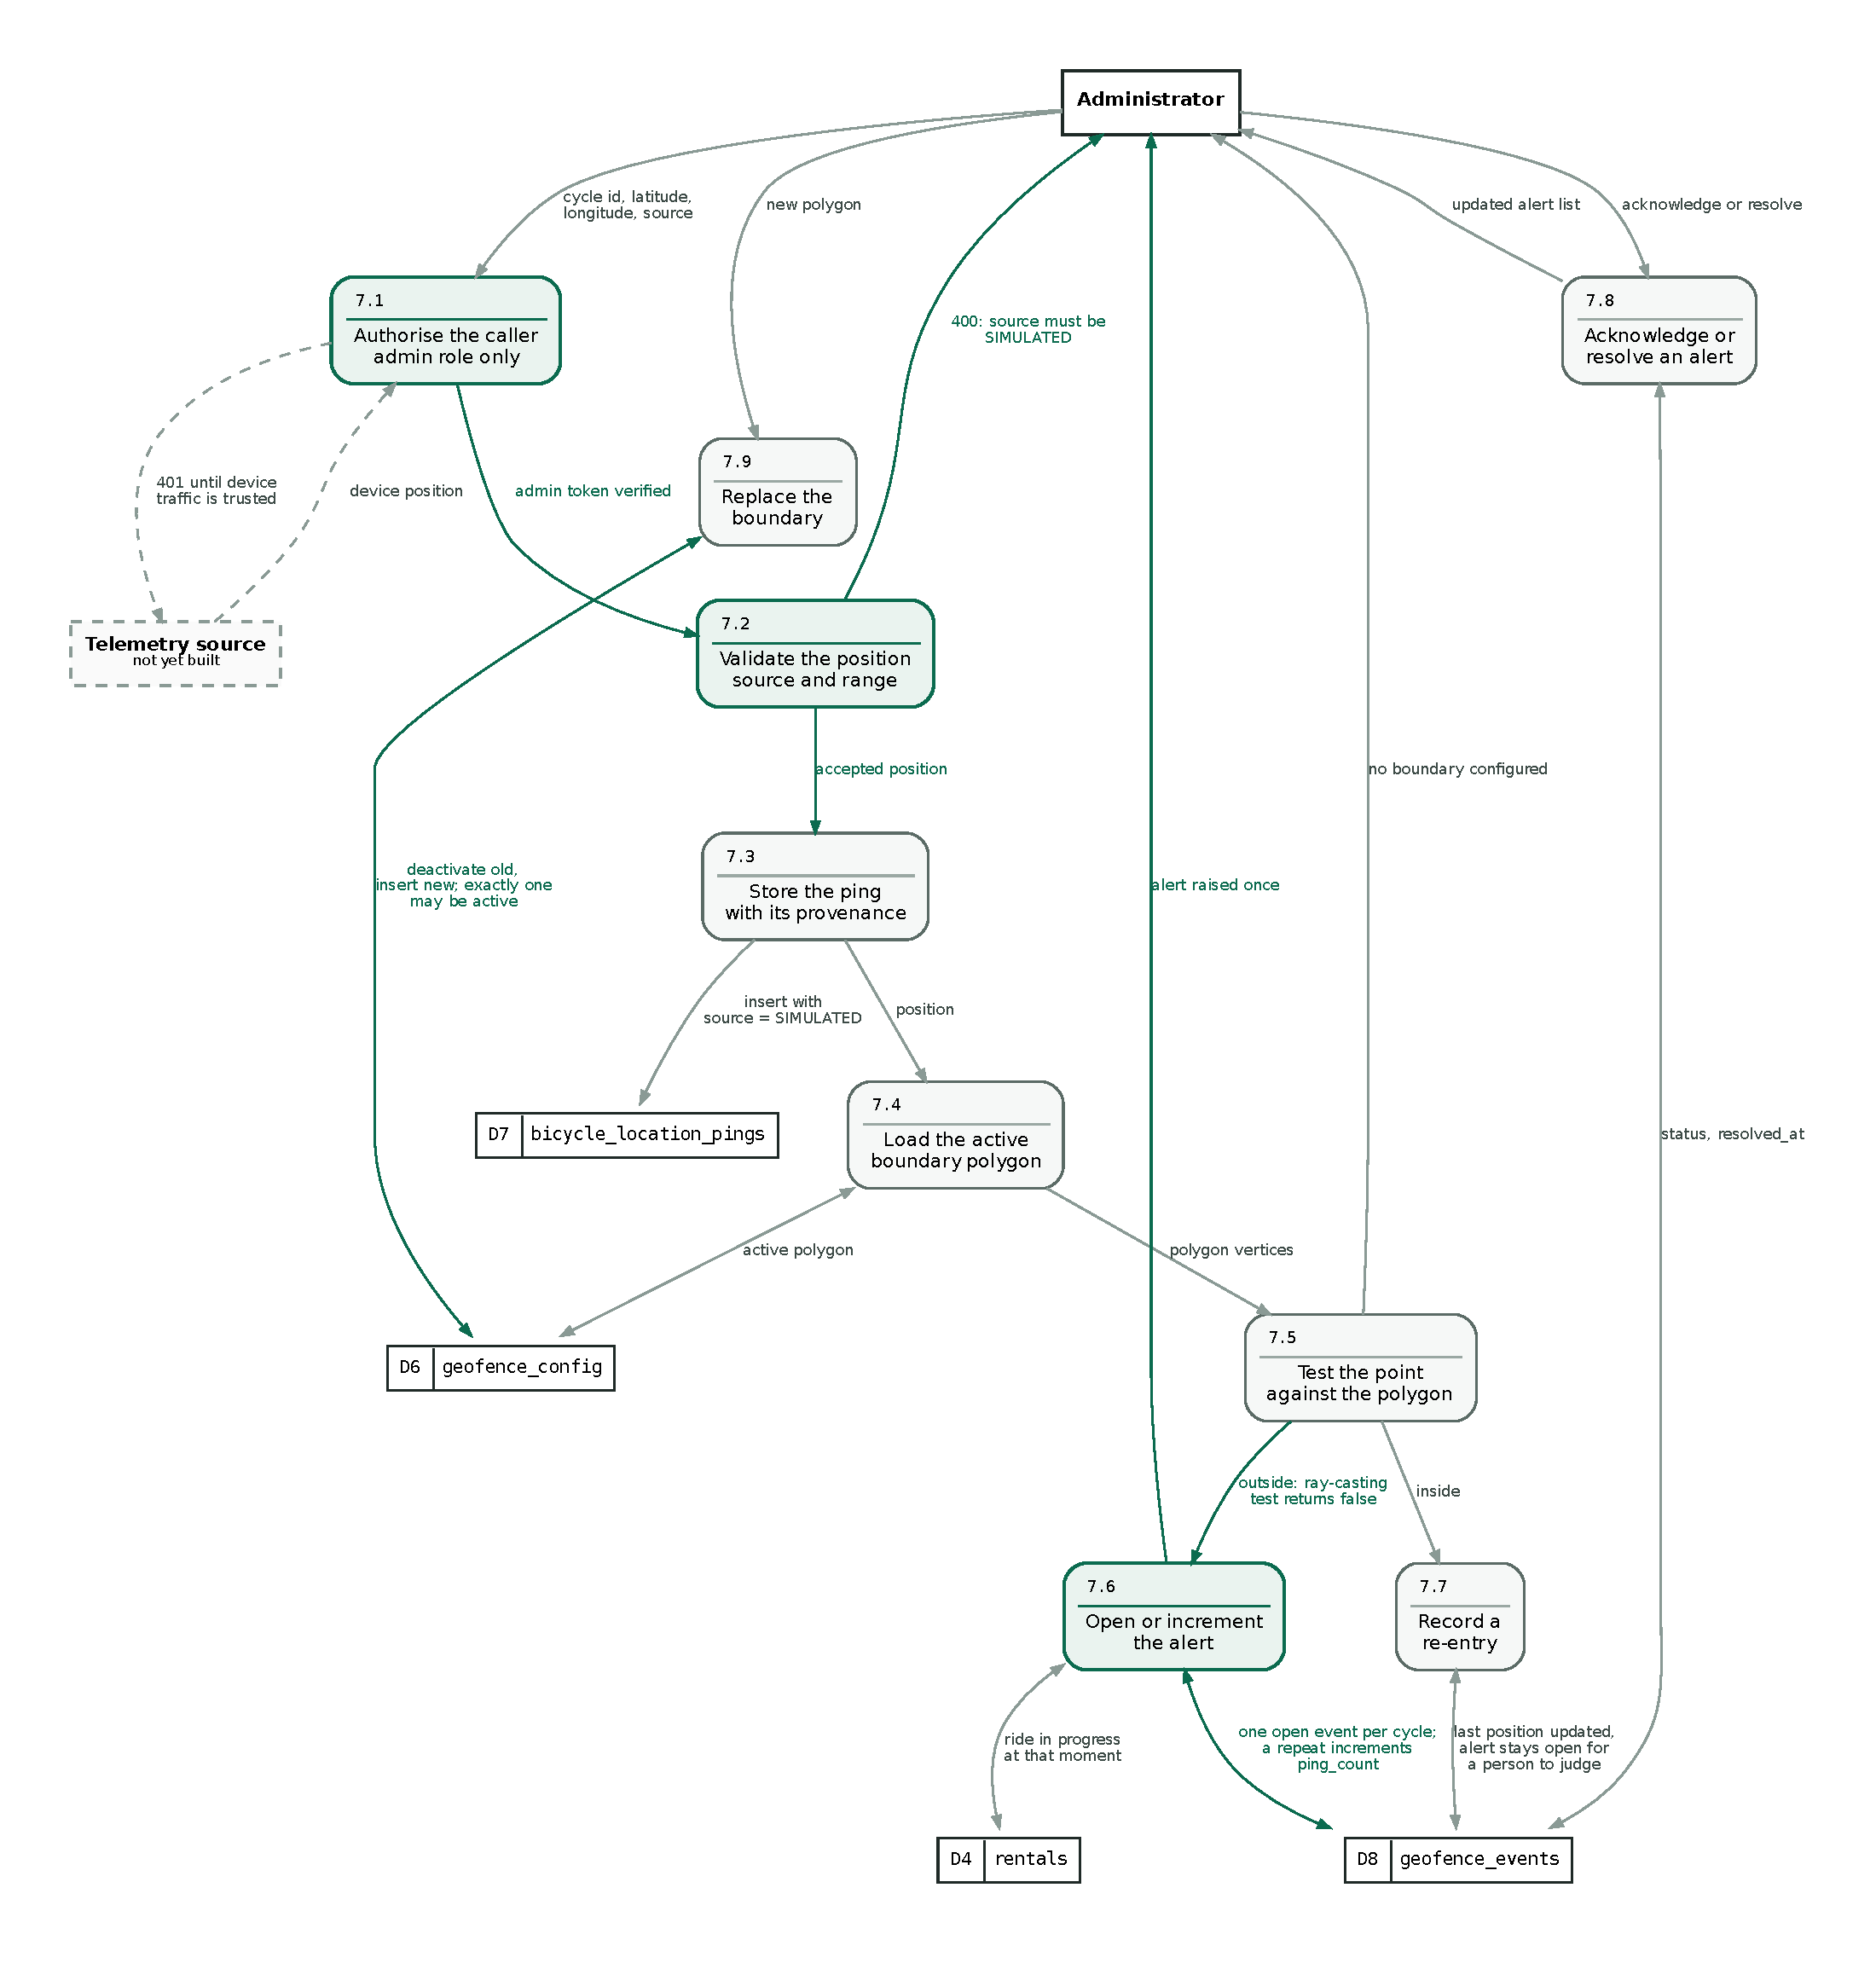
\includegraphics[width=\textwidth]{figures/dfd-l2-geofence.pdf}
  \caption{Level-2 diagram for process 7.0,
    geofencing. Process 7.6 is where the
    de-duplication invariant lives: a repeated breach
    increments an existing alert instead of opening a
    second one.}
  \label{fig:dfd2g}
\end{figure}

\subsection{Level 2: Analytics}

Figure~\ref{fig:dfd2a} explodes process~8.0, and makes
visible the distinction the dashboard draws between
figures that the date filter affects and figures it
does not. Process 8.4 exists for a single reason: to
turn a set of days on which something happened into a
continuous axis that includes the days on which
nothing did.

\begin{sidewaysfigure}
  \centering
  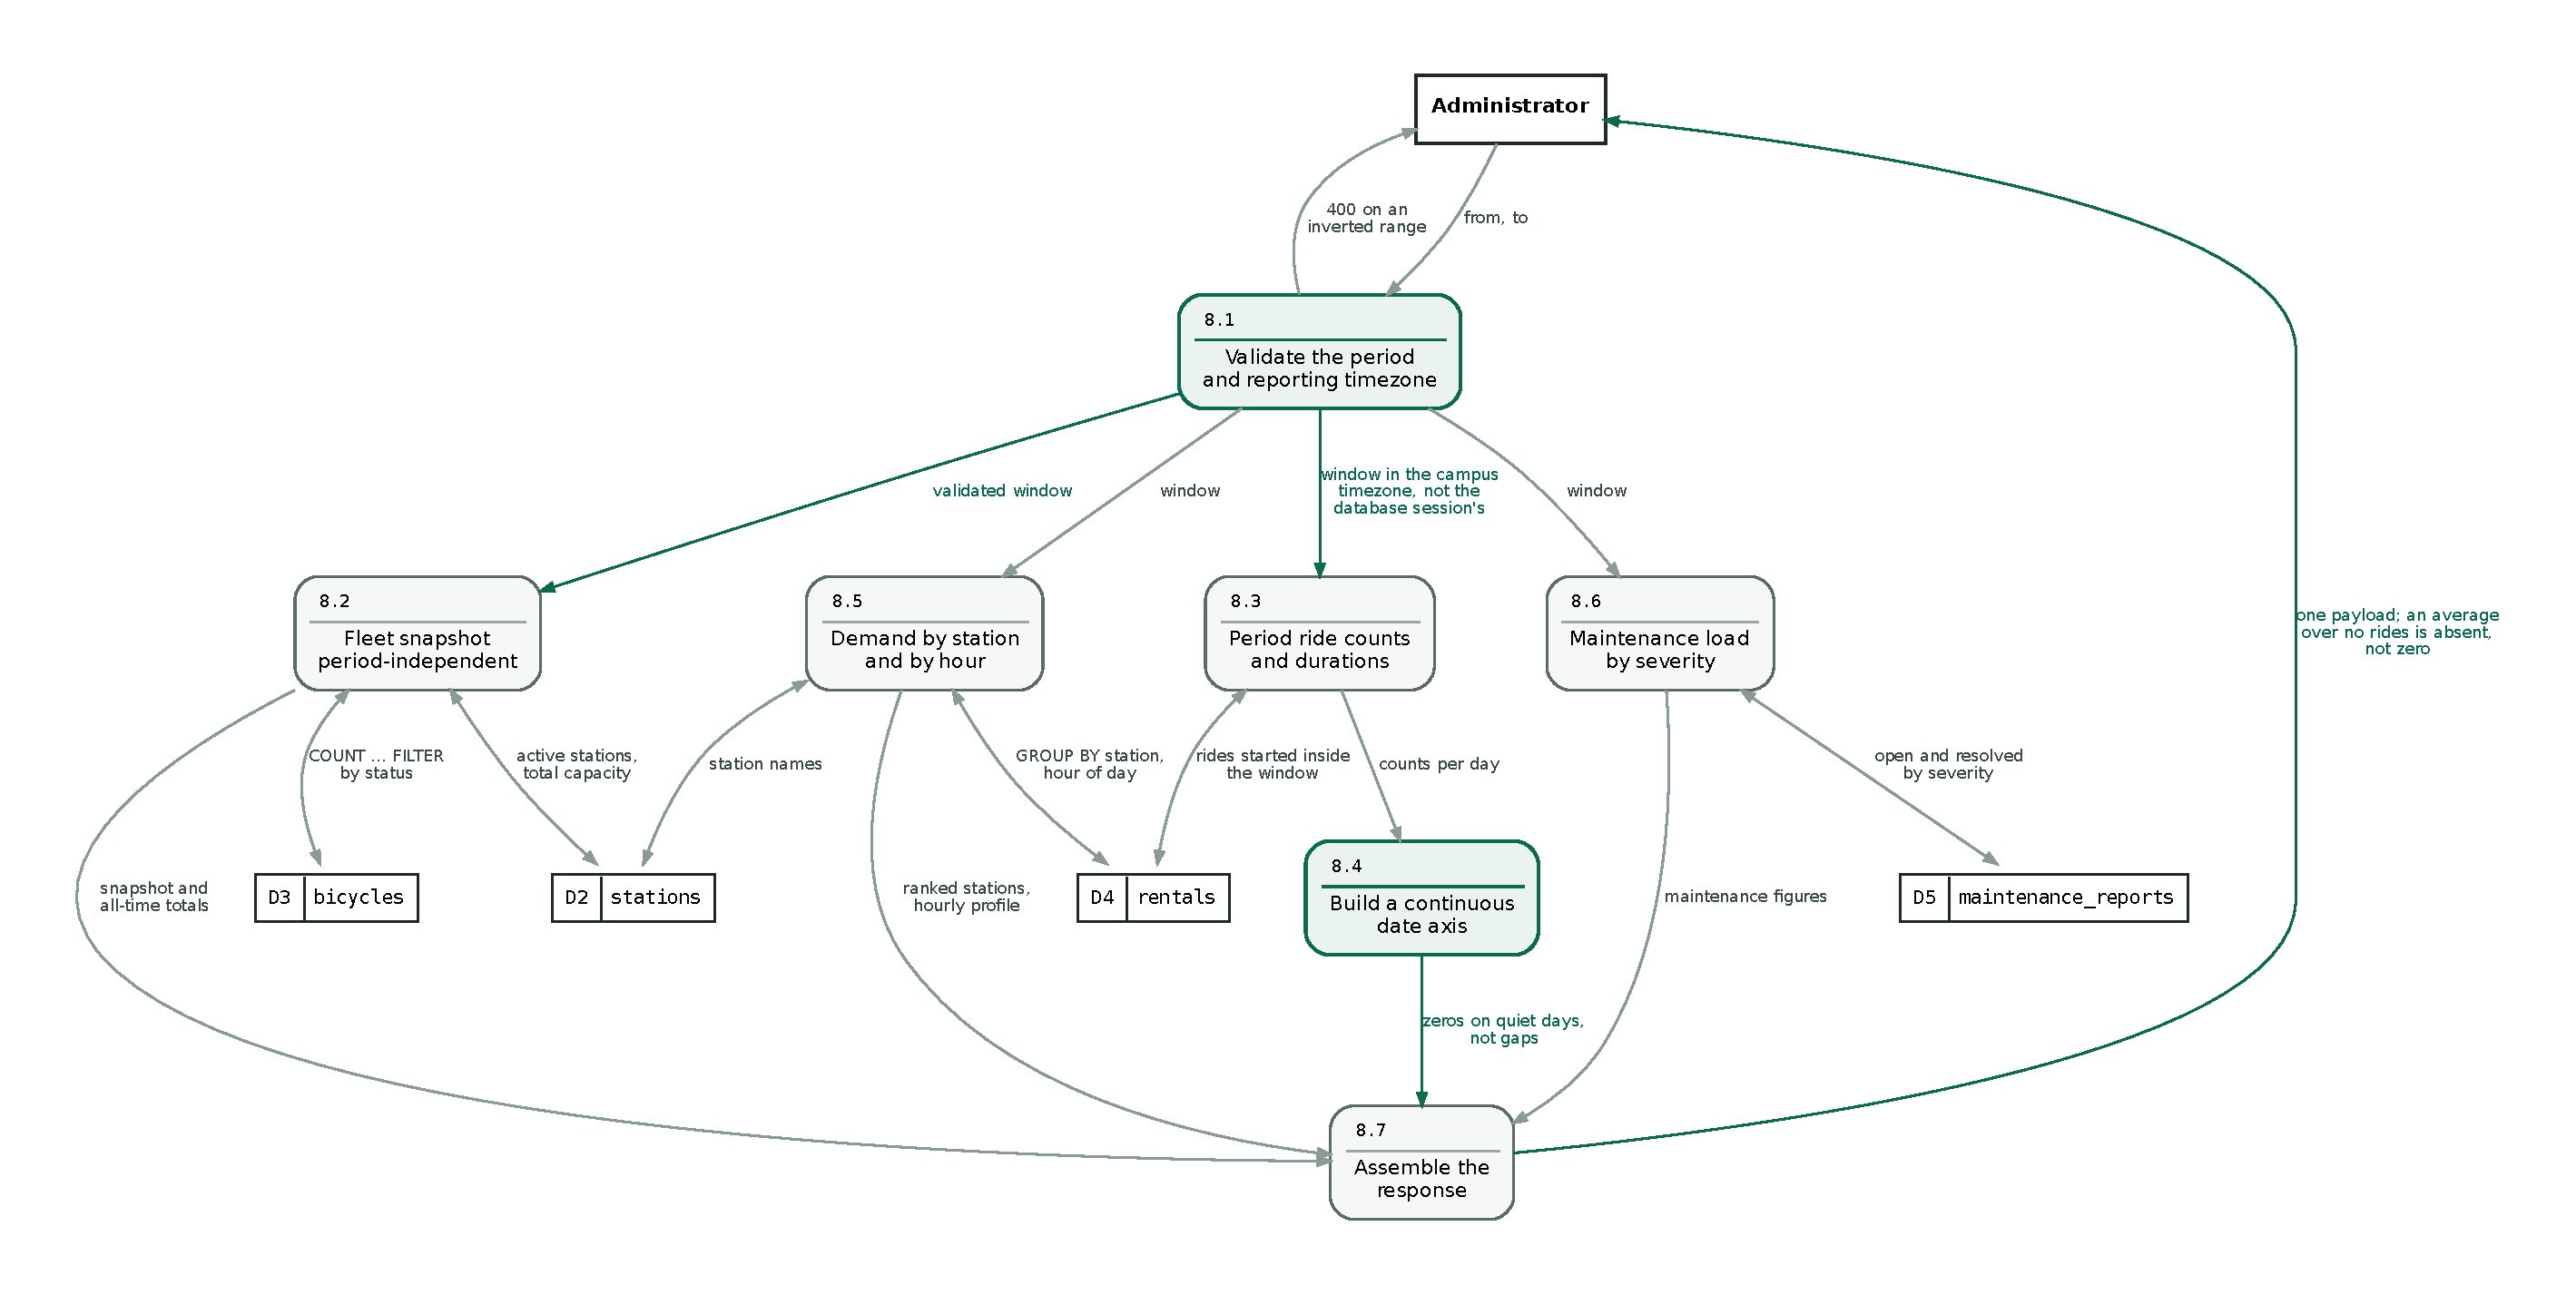
\includegraphics[width=\textheight,height=\textwidth,keepaspectratio]{figures/dfd-l2-analytics.pdf}
  \caption{Level-2 diagram for process 8.0, analytics.
    Snapshot figures (8.2) ignore the selected period;
    period figures (8.3, 8.5, 8.6) do not.}
  \label{fig:dfd2a}
\end{sidewaysfigure}

\subsection{Level 2: Route Planning}

Figure~\ref{fig:dfd2p} explodes process~9.0. The road
graph is built once at start-up rather than per
request (9.1, 9.2); a request resolves two stops,
snaps each onto the network, and runs a shortest-path
search over the traced roads.

\begin{figure}[p]
  \centering
  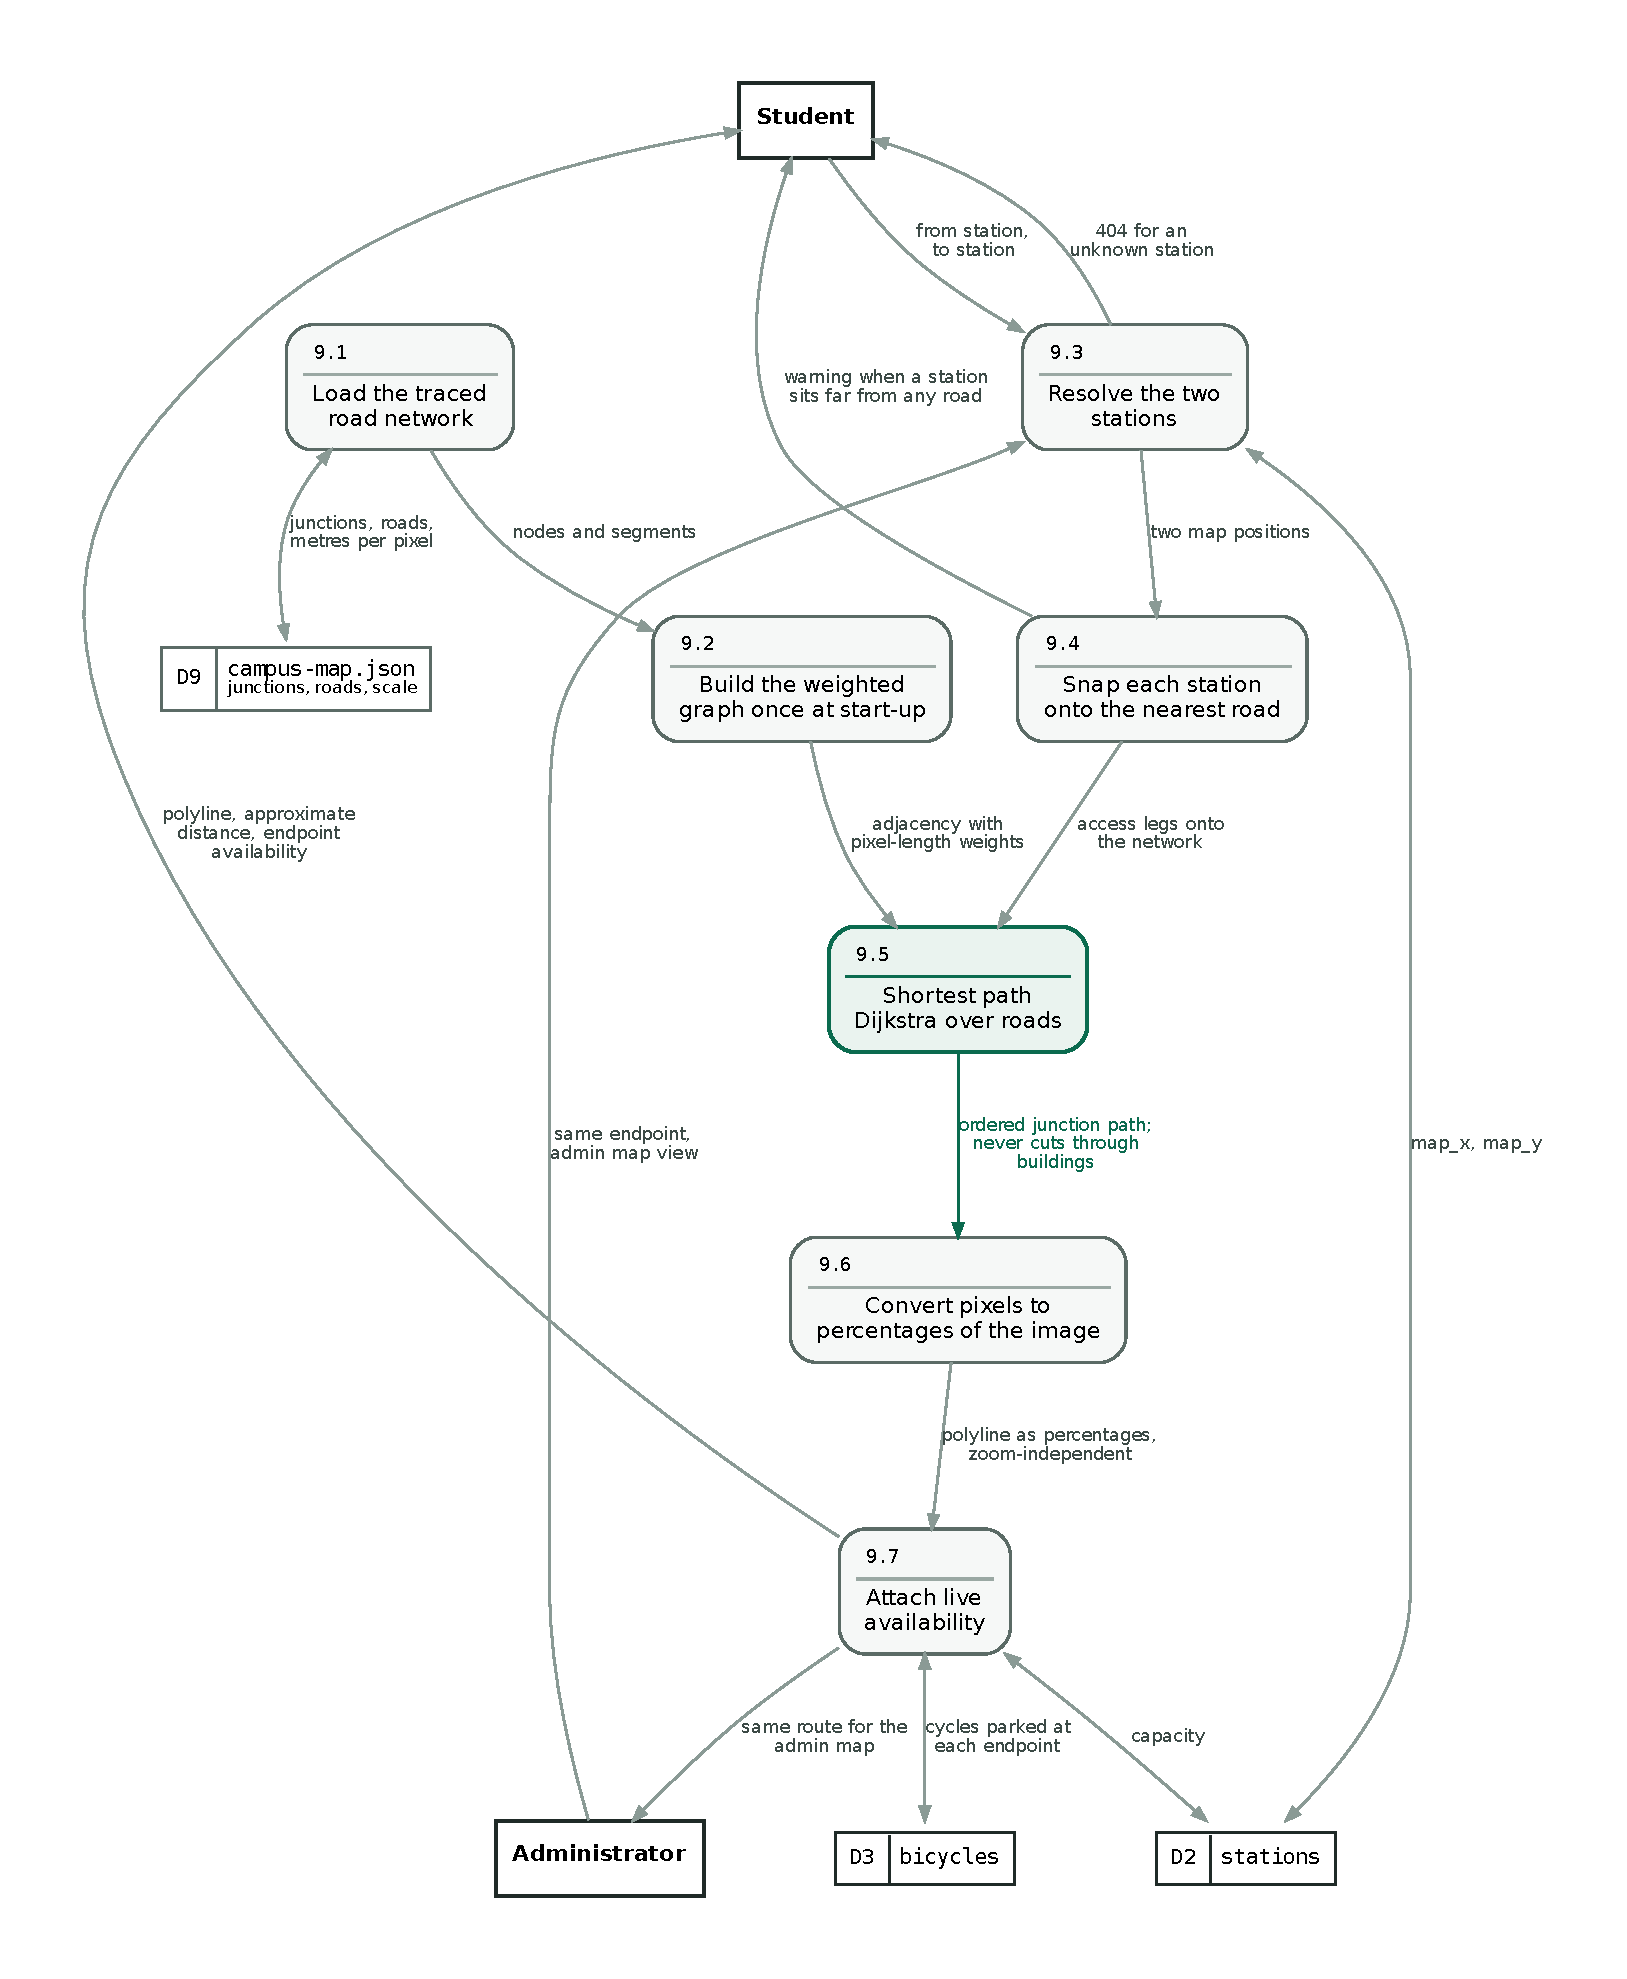
\includegraphics[width=\textwidth]{figures/dfd-l2-route.pdf}
  \caption{Level-2 diagram for process 9.0, route
    planning. The output is expressed as percentages
    of the map image rather than pixels, so that one
    stored route draws correctly at any zoom level.}
  \label{fig:dfd2p}
\end{figure}

\section{Database Design}

\subsection{Tables}

The schema is eight tables: four from Phase~1 and four
added by Phase~2 (Table~\ref{tab:schema}). Phase~3
added columns rather than tables. Primary keys are
\texttt{INTEGER GENERATED ALWAYS AS IDENTITY}, every
enumerated column is constrained by a \texttt{CHECK}
that mirrors a constant in the application code, and
an \texttt{updated\_at} trigger maintains modification
timestamps.

\begin{table}[htbp]
\centering
\begin{tabular}{@{}llp{6.1cm}@{}}
\toprule
\textbf{Table} & \textbf{Phase} & \textbf{Contents} \\
\midrule
\texttt{users} & 1 &
  Accounts, bcrypt password hash~\cite{bcrypt}, role \\
\texttt{stations} & 1 &
  Name, location, capacity, status; latitude and
  longitude added in Phase~2; short code and map
  position added in Phase~3 \\
\texttt{bicycles} & 1 &
  Cycle code, QR code, current stop, status \\
\texttt{rentals} & 1 &
  Rider, cycle, start and end stop, timestamps,
  status \\
\texttt{maintenance\_reports} & 2 &
  Reported fault, severity, lifecycle status,
  reporter, resolution \\
\texttt{geofence\_config} & 2 &
  Campus boundary polygon stored as JSONB \\
\texttt{bicycle\_location\_pings} & 2 &
  Every submitted position, with its source \\
\texttt{geofence\_events} & 2 &
  Boundary violations, de-duplicated per cycle \\
\bottomrule
\end{tabular}
\caption{Database tables.}
\label{tab:schema}
\end{table}

\subsection{Invariants Enforced in the Database}
\label{sec:concurrency}

Rules that must hold under concurrent use are pushed
into the database, because application-level checks of
the form \emph{read, decide, then write} are unsafe
when two requests interleave between the read and the
write~\cite{bernstein1987}. The schema therefore
carries:

\begin{itemize}
  \item \texttt{uq\_active\_rental\_per\_user} and
    \texttt{uq\_active\_rental\_per\_bicycle} ---
    partial unique indexes making a second active
    rental impossible rather than merely unlikely;
  \item \texttt{uq\_geofence\_open\_event\_per\_bicycle}
    --- the same device applied to alerts, which is
    what prevents a cycle left outside the boundary
    from generating an unbounded number of them;
  \item \texttt{uq\_geofence\_single\_active} --- at
    most one active boundary configuration;
  \item \texttt{chk\_ended\_at} and
    \texttt{chk\_maintenance\_resolved} --- a
    completed ride must carry an end timestamp, and a
    resolved report a resolution time;
  \item \texttt{chk\_bicycle\_in\_use\_unparked} and
    \texttt{chk\_bicycle\_parked\_has\_station} --- a
    cycle in use is parked nowhere, and a cycle
    available or reserved is parked somewhere;
  \item \texttt{chk\_stations\_coords\_paired},
    \texttt{chk\_stations\_map\_paired} and the
    accompanying range checks --- a stop has both
    coordinates or neither, both map positions or
    neither, and each lies within its valid range.
\end{itemize}

Above these, the service layer takes explicit row
locks. Starting a rental, returning one, filing a
report and changing a bicycle's status all run inside
a transaction that holds \texttt{SELECT \ldots{} FOR
UPDATE} on the bicycle row, so those four operations
are serialised against each other for a given cycle.
The database constraints remain as a second line of
defence, and the unique-violation error codes they
raise are translated into readable messages rather
than surfacing as failures. In total the schema
carries 24 indexes and unique constraints.

\subsection{Migrations and Seed Data}
\label{sec:migrations}

Neither Phase~2 nor Phase~3 could rebuild the
database, because an instance already held accounts
and rental history. Each schema change is therefore
delivered as an additive, idempotent migration: it
adds columns and tables, creates constraints only when
they are absent, and never drops or truncates
anything. Running a migration twice has the same
effect as running it once. Separate, equally
idempotent seed scripts fill in stop coordinates and
map positions, install a campus boundary, and add
demonstration maintenance reports only when that table
is still empty, so that a database holding genuine
reports is left untouched.

\section{Implementation Details}

\subsection{Authentication and Access Control}

Passwords are hashed with bcrypt~\cite{bcrypt} at a
configurable cost factor; the hash never leaves the
database layer. A successful sign-in returns a JWT
carrying the user id and role, which the browser
attaches to every subsequent request.

Two decisions here are deliberate. First, public
registration always creates a student: there is no
input through which a caller can request the
administrator role, which removes privilege escalation
by construction. Second, and more pervasively,
\textbf{the identity used for authorisation is always
taken from the verified token, never from the request
body or query string}. A request for ride history
carries no user id at all; the server derives it. This
single convention is what makes objective~5 hold
across every endpoint rather than endpoint by
endpoint.

\subsection{Rentals and the Return Workflow}

A rental begins when a student submits a QR code. In
one transaction, the service checks that the student
holds no active ride, locks and loads the bicycle by
its QR code, verifies that it is available and free of
any safety hold, creates the rental, and marks the
bicycle \texttt{IN\_USE} with no stop --- a cycle in
use is parked nowhere. The return reverses this: the
ride is completed with an end stop and timestamp, and
the bicycle is parked at that stop.

Capacity is enforced when an administrator assigns
cycles to a stop, but never on return. A student must
always be able to end a ride; refusing a return
because a stop is notionally full would strand them.

\subsection{The Campus Map and Route Planning}
\label{sec:map}

The prototype drew stops on OpenStreetMap tiles. Two
problems made that the wrong basemap for this system.
Tiles require internet access at the moment the page
is opened, which a demonstration cannot rely on; and
an open street map of the area shows the campus
largely as unlabelled polygons, so a marker on it
tells a student nothing about which building they are
standing next to.

Phase~3 replaced it with the illustrated campus map
that students already recognise
(Figure~\ref{fig:uimap}). The artwork is not
georeferenced, so the implementation deliberately does
not treat it as though it were: Leaflet runs in
\texttt{CRS.Simple} mode with the image as the only
layer, and every position --- stops, route vertices
--- is a percentage of the image width and height,
which is exactly what the database stores in
\texttt{stations.map\_x} and \texttt{map\_y}. Markers
therefore stay on their building at any container size
and zoom level. The geographic latitude and longitude
columns added in Phase~2 are retained and still used
by the geofencing module, which does need real
coordinates; the two coordinate systems are kept
separate rather than conflated.

\begin{figure}[htbp]
  \centering
  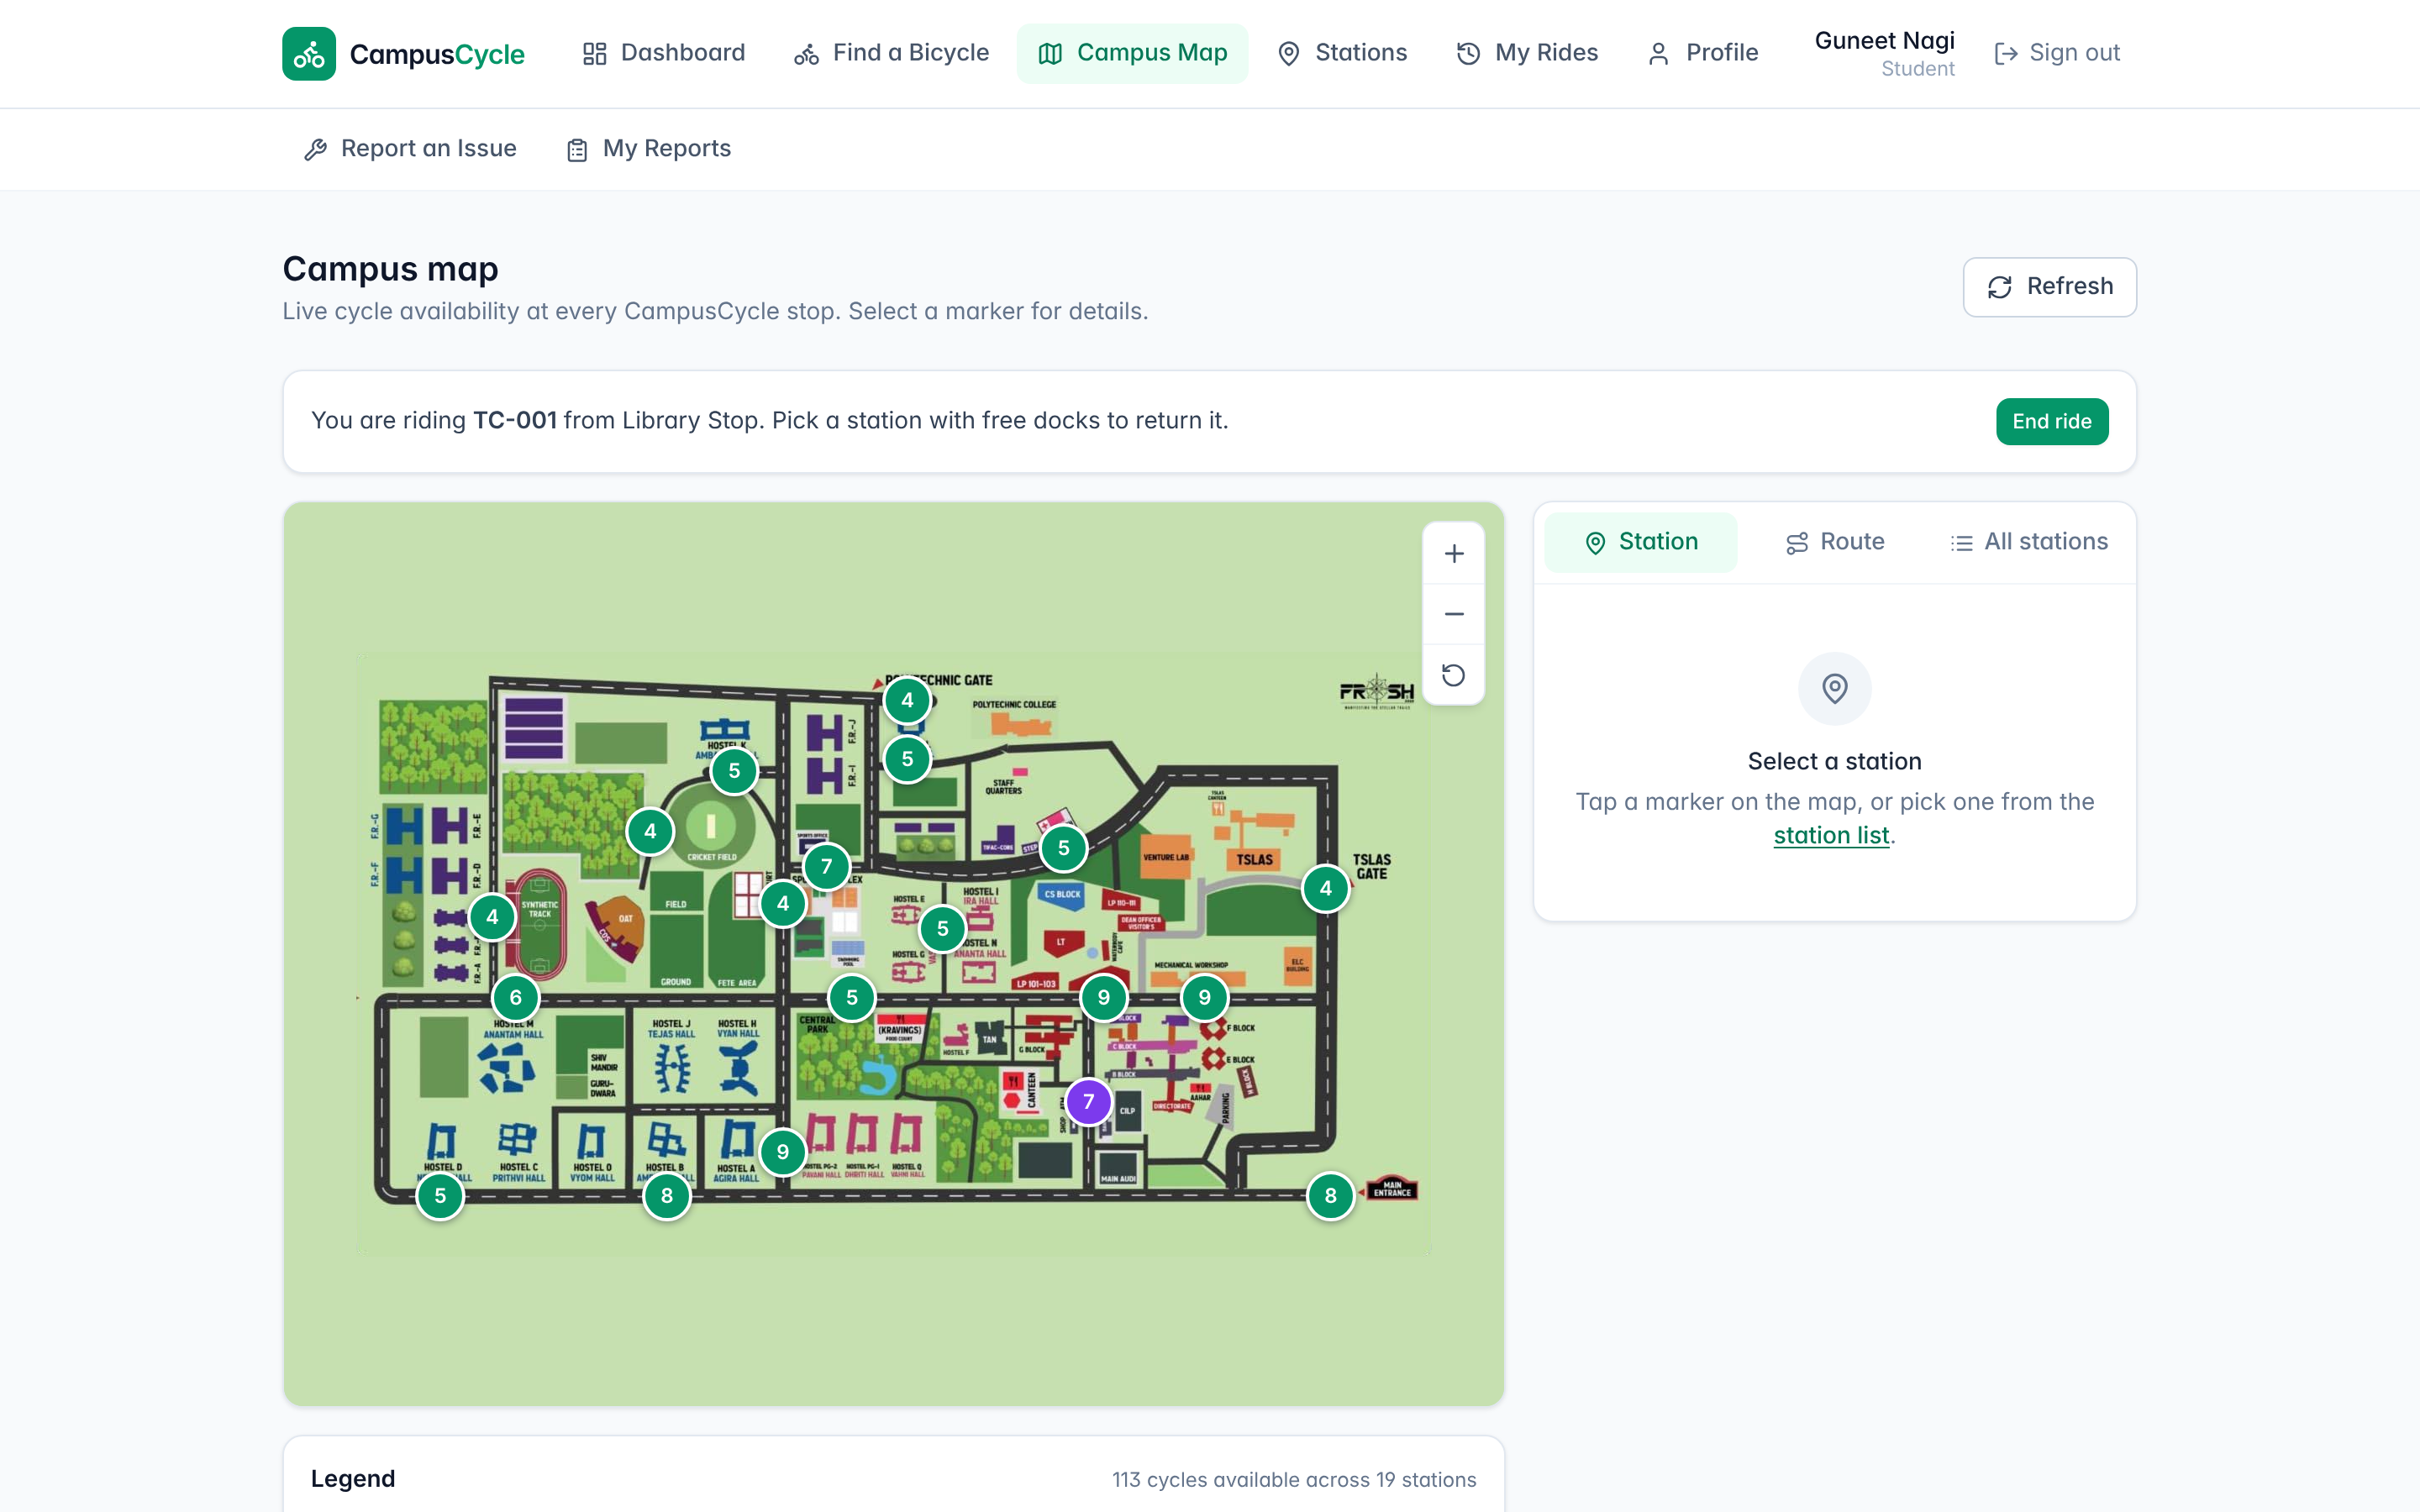
\includegraphics[width=\textwidth]{figures/ui-student-map.png}
  \caption{Student campus map. One marker per stop,
    numbered and coloured by live availability, drawn
    over the illustrated campus map. The banner at the
    top is the student's ride in progress.}
  \label{fig:uimap}
\end{figure}

On top of the map sits route planning. The roads drawn
on the illustration were traced by hand into a
configuration file as a set of junctions and
polylines, in the pixel coordinates of the image. At
start-up the service builds a weighted graph from that
file once. A route request then snaps each stop onto
the nearest road segment, runs Dijkstra's shortest
path algorithm~\cite{dijkstra1959} over the traced
roads, and returns the resulting polyline as
percentages of the image
(Figure~\ref{fig:uiroute}). Routes therefore follow
the drawn roads and never cut through buildings.

Two honesty constraints are built into the output.
Distances are computed from the path length in pixels
multiplied by the documented map scale, and are
reported as approximate, because the artwork is an
illustration and not a survey. No travel time is
estimated at all, since that would require a cycling
speed the system has no basis for assuming.

\begin{figure}[htbp]
  \centering
  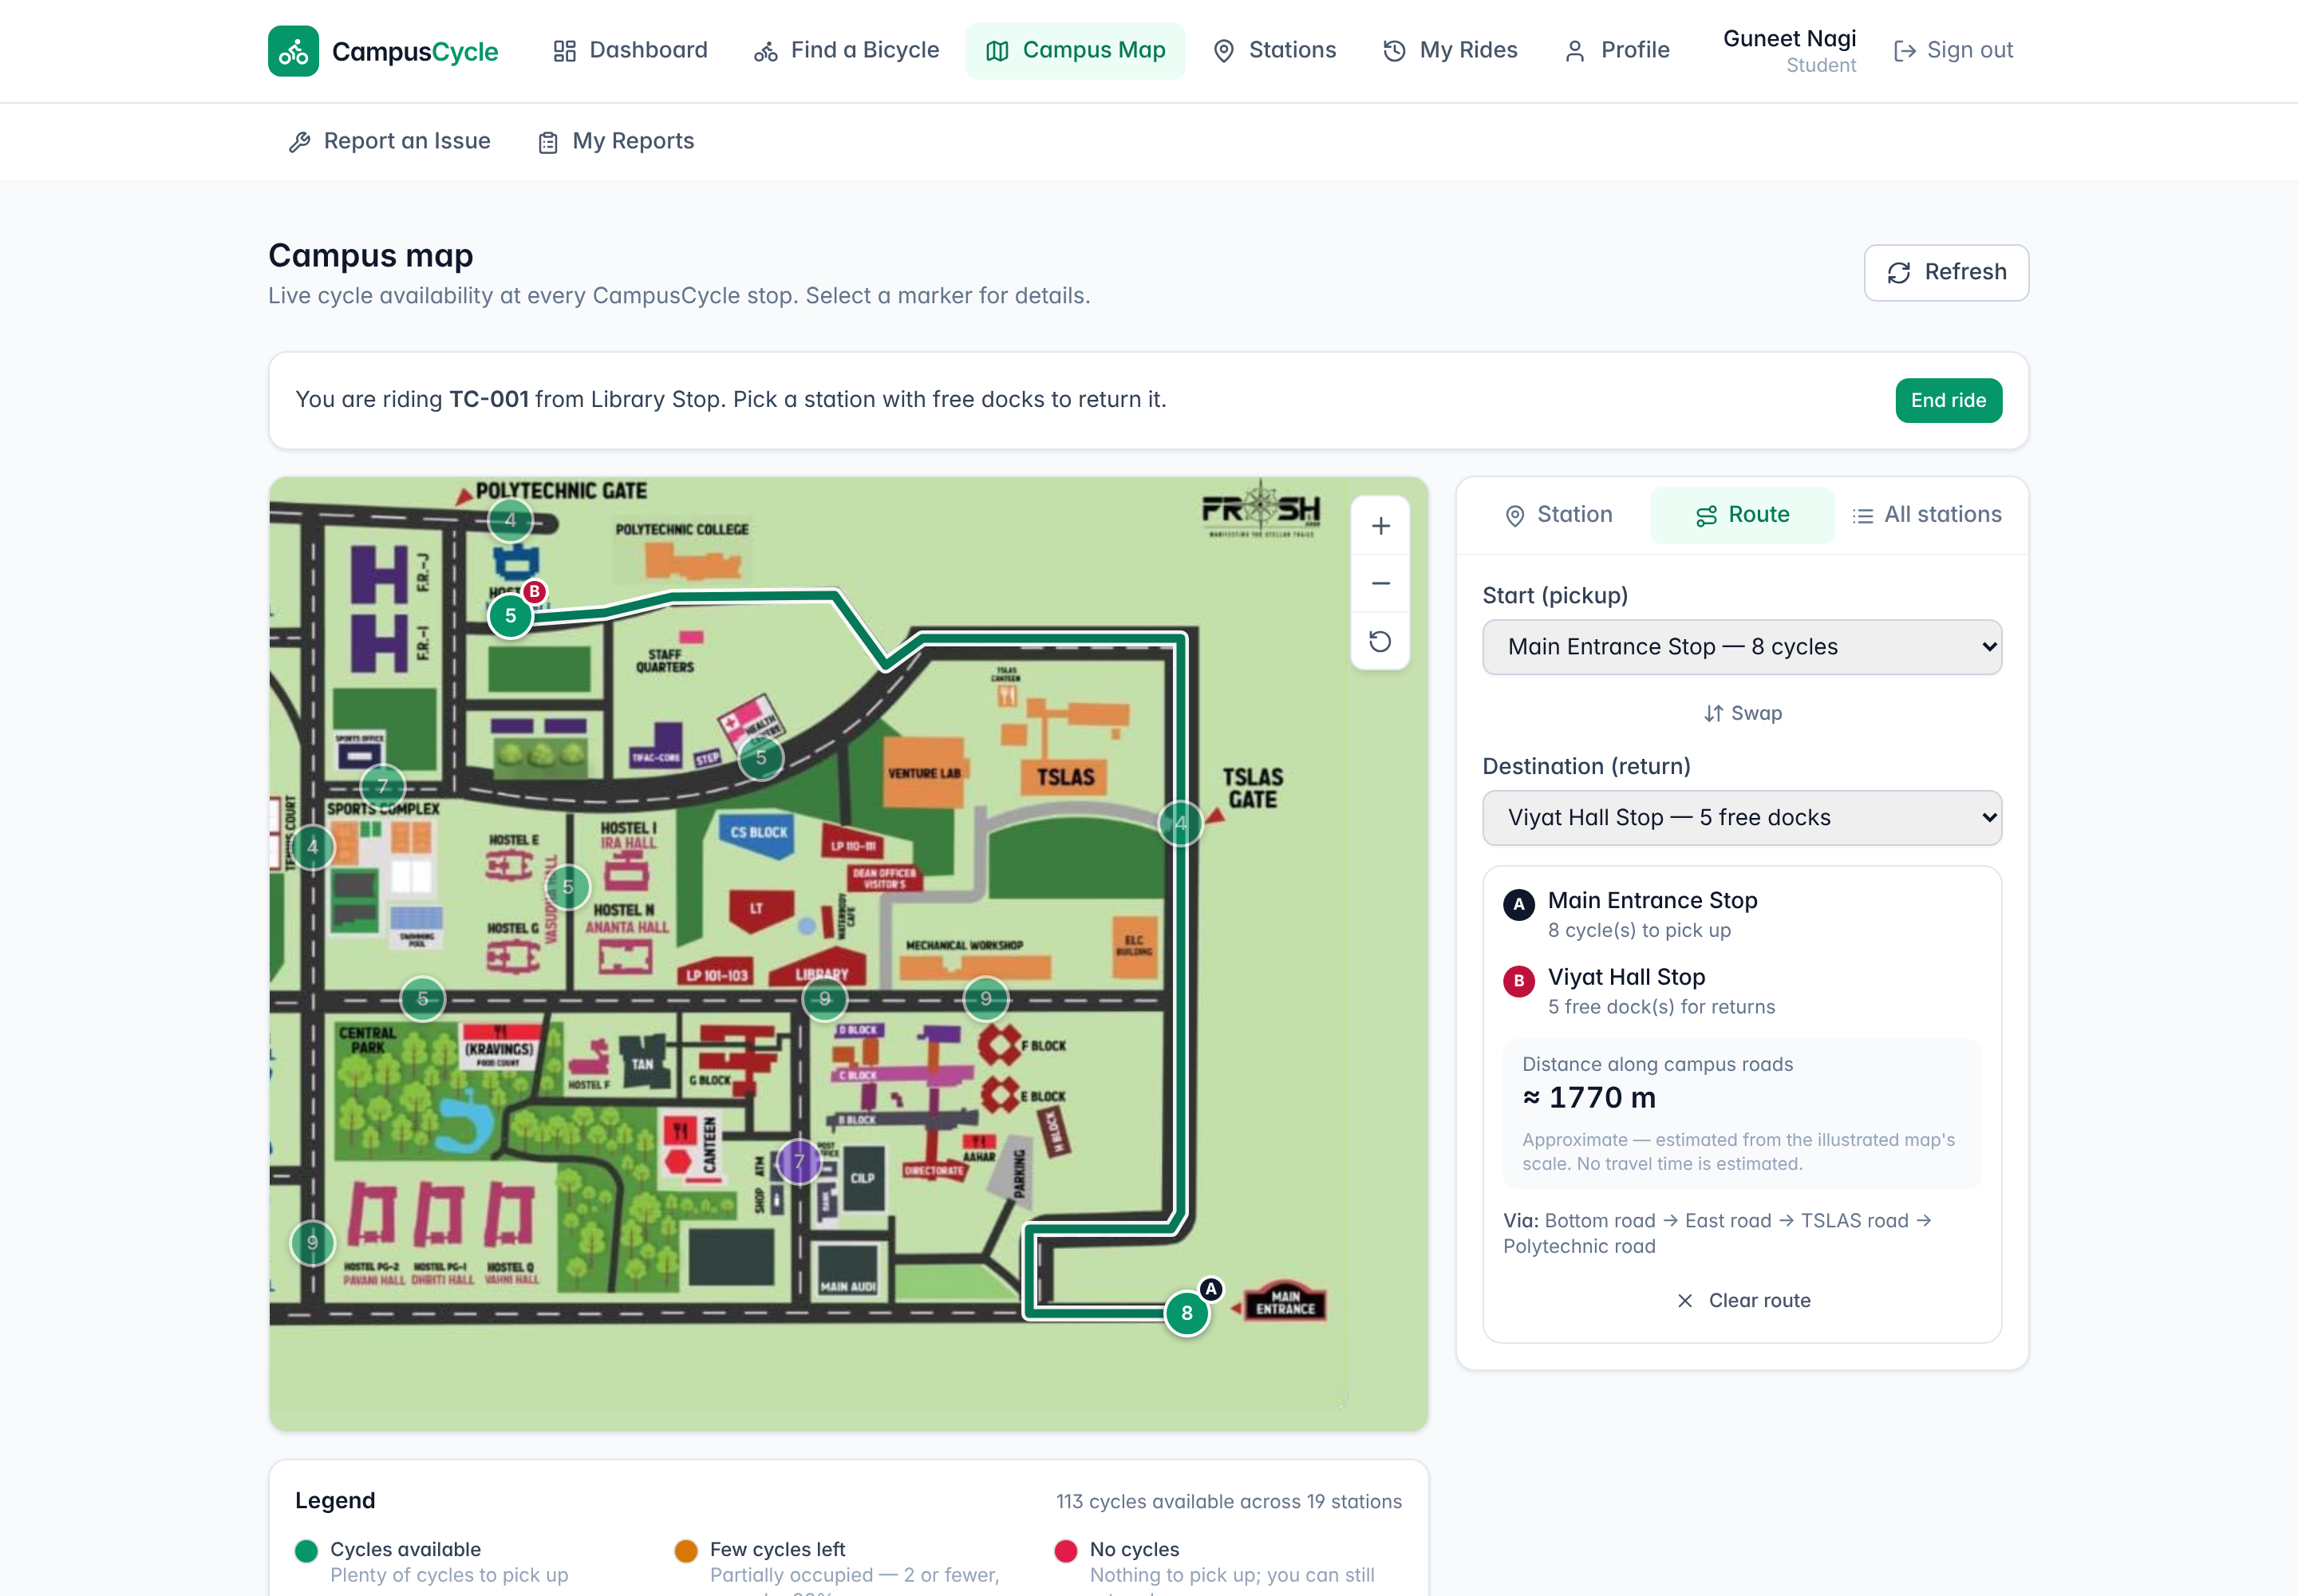
\includegraphics[width=\textwidth]{figures/ui-student-route.png}
  \caption{A planned route between two stops. The path
    follows the roads traced on the map, the distance
    is labelled as approximate, and the roads used are
    named. Endpoint availability --- cycles to pick up
    at~A, free docks at~B --- is attached to the
    result.}
  \label{fig:uiroute}
\end{figure}

\subsection{Stop Availability}

Availability is defined once, in a single module, and
every surface that displays it --- the stop list, the
stop detail page, the map, the student dashboard ---
derives its figures from that one definition:

\begin{itemize}
  \item \texttt{available\_count}: bicycles with
    status \texttt{AVAILABLE} parked at the stop;
  \item \texttt{availability\_pct}:
    \texttt{available\_count} as a percentage of
    capacity, defined as zero when capacity is zero so
    that no screen can divide by zero;
  \item \texttt{availability\_level}: one of
    \texttt{INACTIVE}, \texttt{NONE}, \texttt{LOW} or
    \texttt{GOOD}. A stop is \texttt{LOW} when at most
    two cycles remain \emph{or} fewer than 20\% of its
    capacity is available --- the count catches a
    nearly-empty large stop, the percentage a
    nearly-empty small one.
\end{itemize}

\subsection{Ride History}

Ride durations are computed by PostgreSQL from the
stored \texttt{TIMESTAMPTZ} values rather than in the
browser: a completed ride reports
\texttt{ended\_at} $-$ \texttt{started\_at}, an active
one reports \texttt{NOW()} $-$ \texttt{started\_at},
and a ride with a missing or inconsistent timestamp
reports no duration at all rather than a negative or
invented one. Administrators additionally get filters
by date range, cycle, stop and status, with
pagination; no endpoint returns an unbounded result
set.

\subsection{Maintenance and the Safety Hold}

A student reports a fault against a cycle with a
category, a description and a severity
(Figure~\ref{fig:uireport}). Severity drives
everything that follows:

\begin{itemize}
  \item A \texttt{HIGH} or \texttt{CRITICAL} report
    places the cycle on a \textbf{safety hold}. If the
    cycle is parked it is moved to
    \texttt{MAINTENANCE} immediately. If it is out on
    a ride the rider is not interrupted --- taking a
    cycle out from under someone mid-ride would be
    worse than the fault --- and the hold is applied
    when it is returned, so it is parked as
    \texttt{MAINTENANCE} rather than
    \texttt{AVAILABLE}.
  \item A \texttt{LOW} or \texttt{MEDIUM} report is
    recorded for review and leaves the cycle in
    service.
\end{itemize}

While a hold exists the cycle cannot be rented, cannot
be parked as available on return, and cannot be forced
back into service by an administrator. All three
routes consult the same check. Reports move through
\texttt{OPEN} $\rightarrow$ \texttt{IN\_PROGRESS}
$\rightarrow$ \texttt{RESOLVED} $\rightarrow$
\texttt{CLOSED}, with reopening permitted from the two
middle states and \texttt{CLOSED} terminal; invalid
transitions are refused, and resolution notes are
required to resolve or close a report
(Figure~\ref{fig:uimaint}).

Resolving a report does \emph{not} by itself return
the cycle to service. Clearing a report is a statement
about a record; returning a cycle to service is a
statement about a physical object that someone must
have actually repaired and parked. The system
therefore requires a separate, explicit administrative
action, and permits it only once no hold remains.

\begin{figure}[htbp]
  \centering
  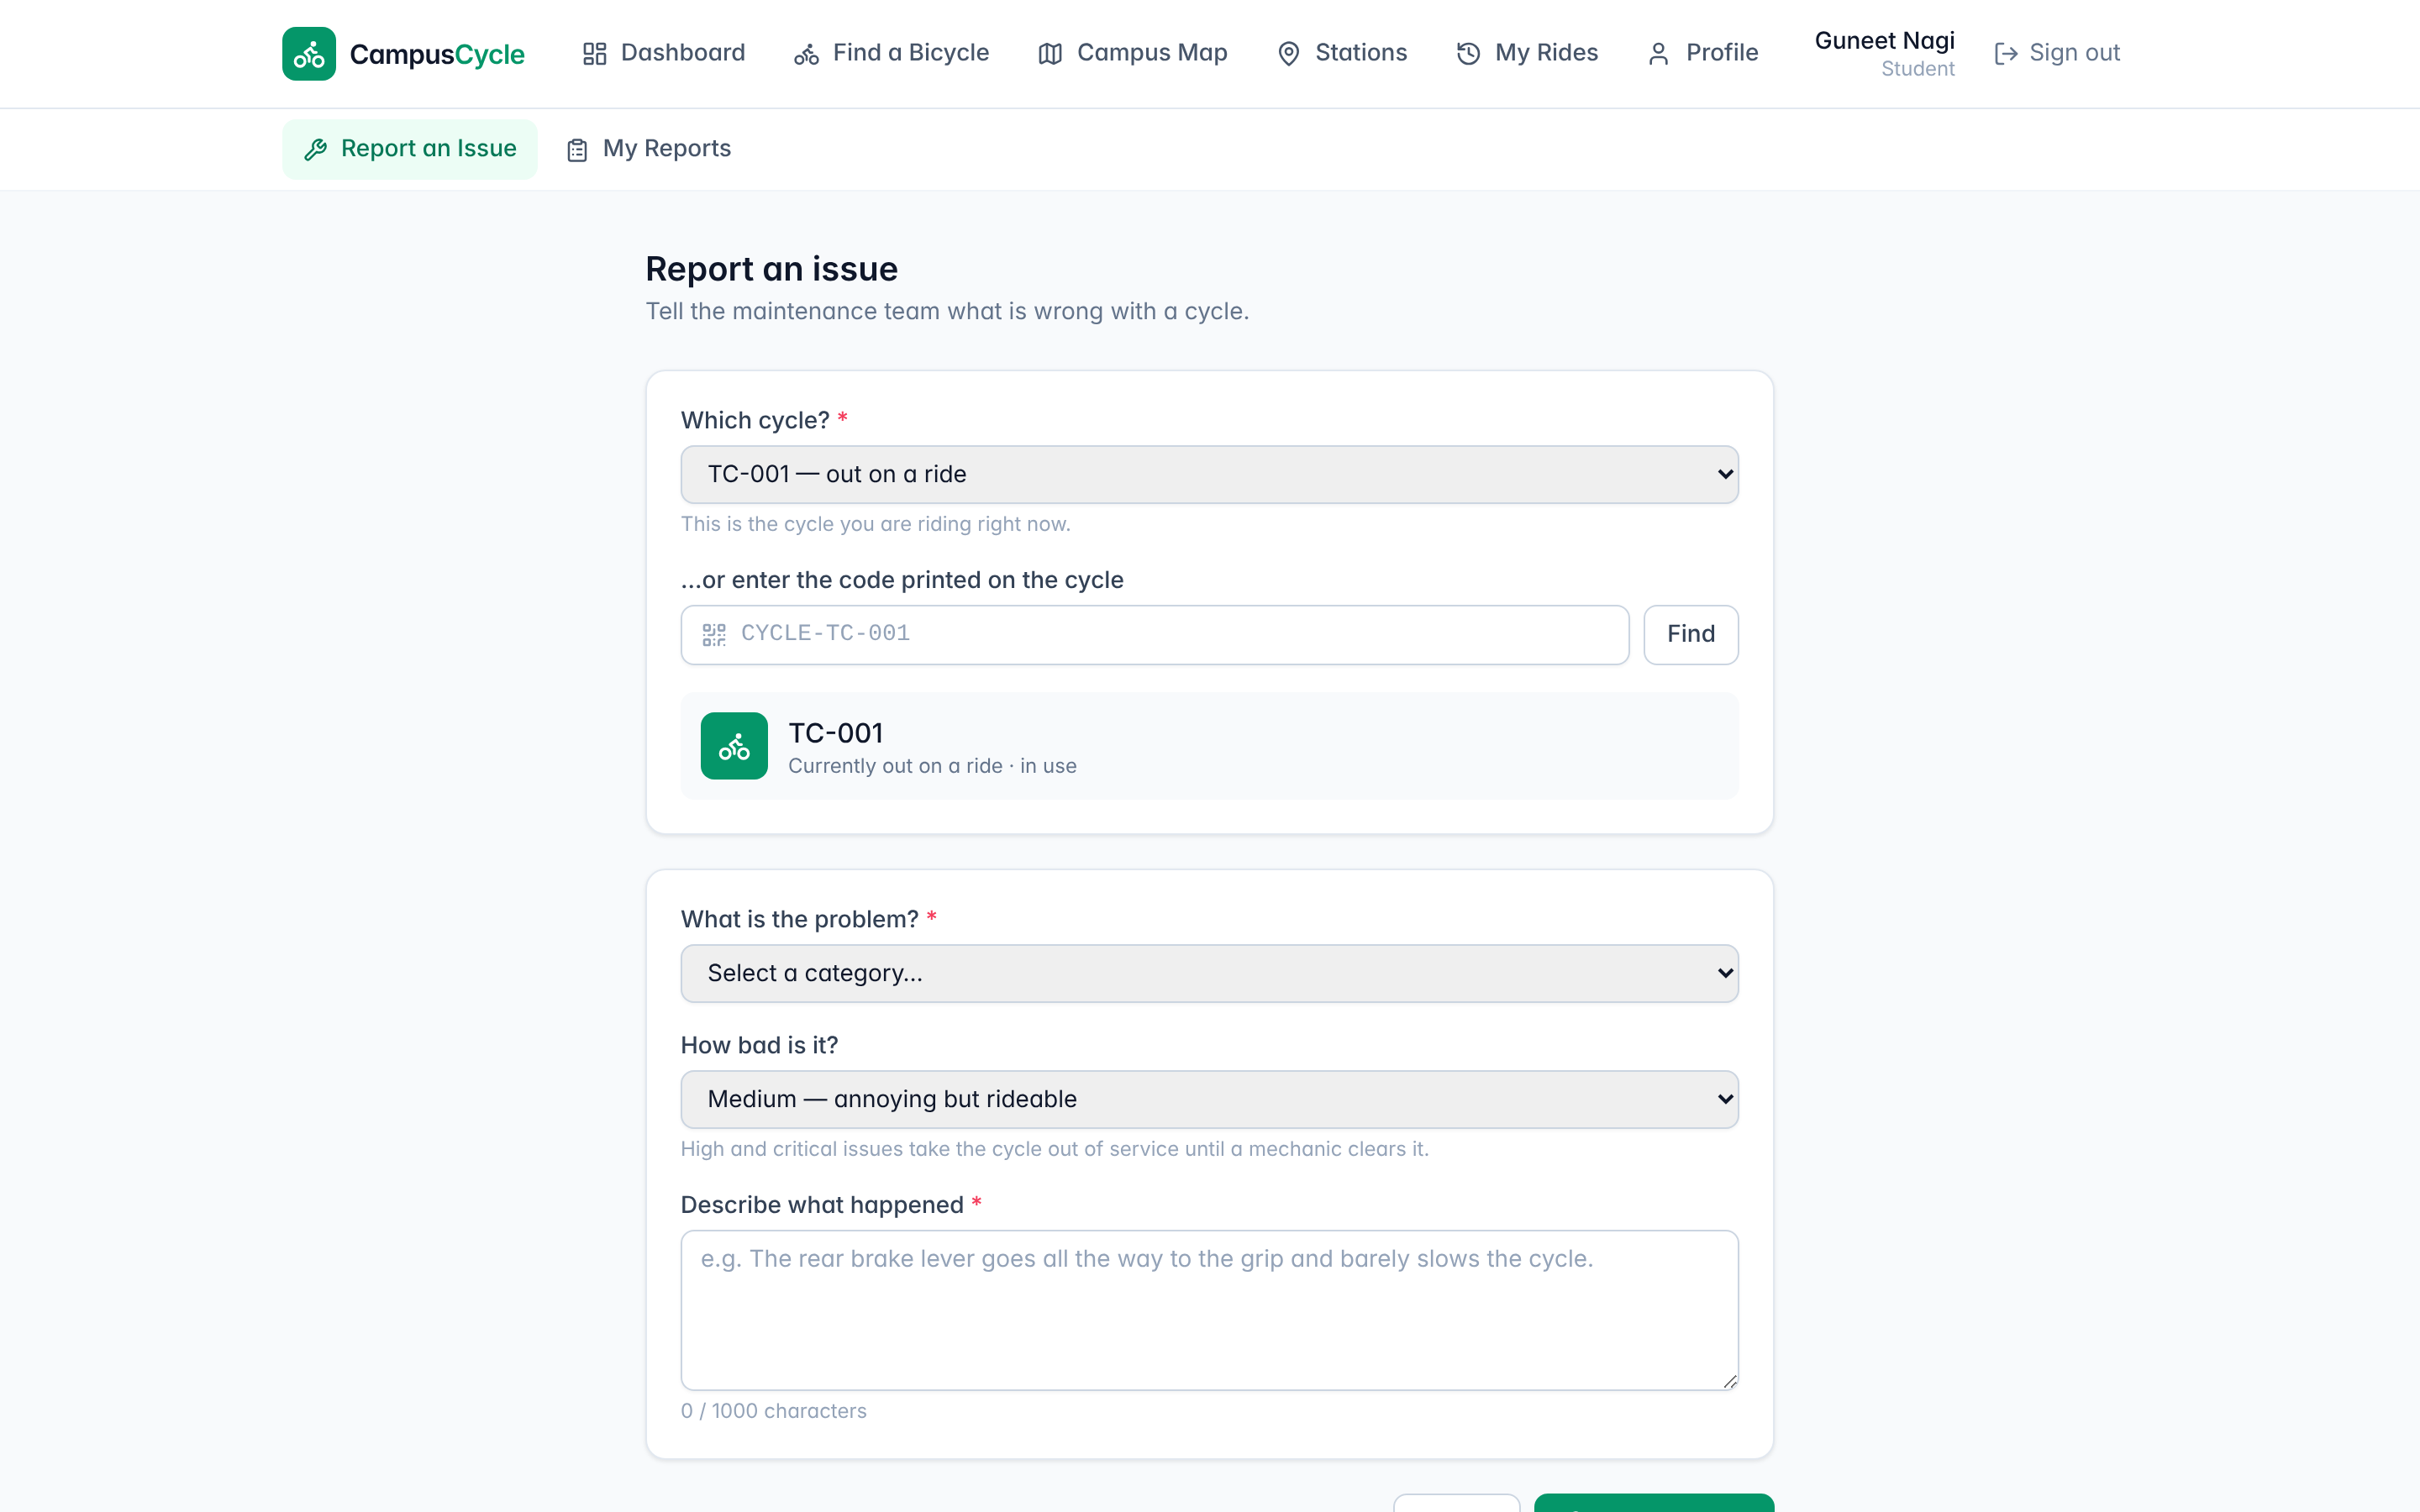
\includegraphics[width=0.92\textwidth]{figures/ui-student-report.png}
  \caption{Fault reporting. The cycle is pre-selected
    from the student's active ride, and the form warns
    that a safety-severity report takes the cycle out
    of service.}
  \label{fig:uireport}
\end{figure}

\begin{figure}[htbp]
  \centering
  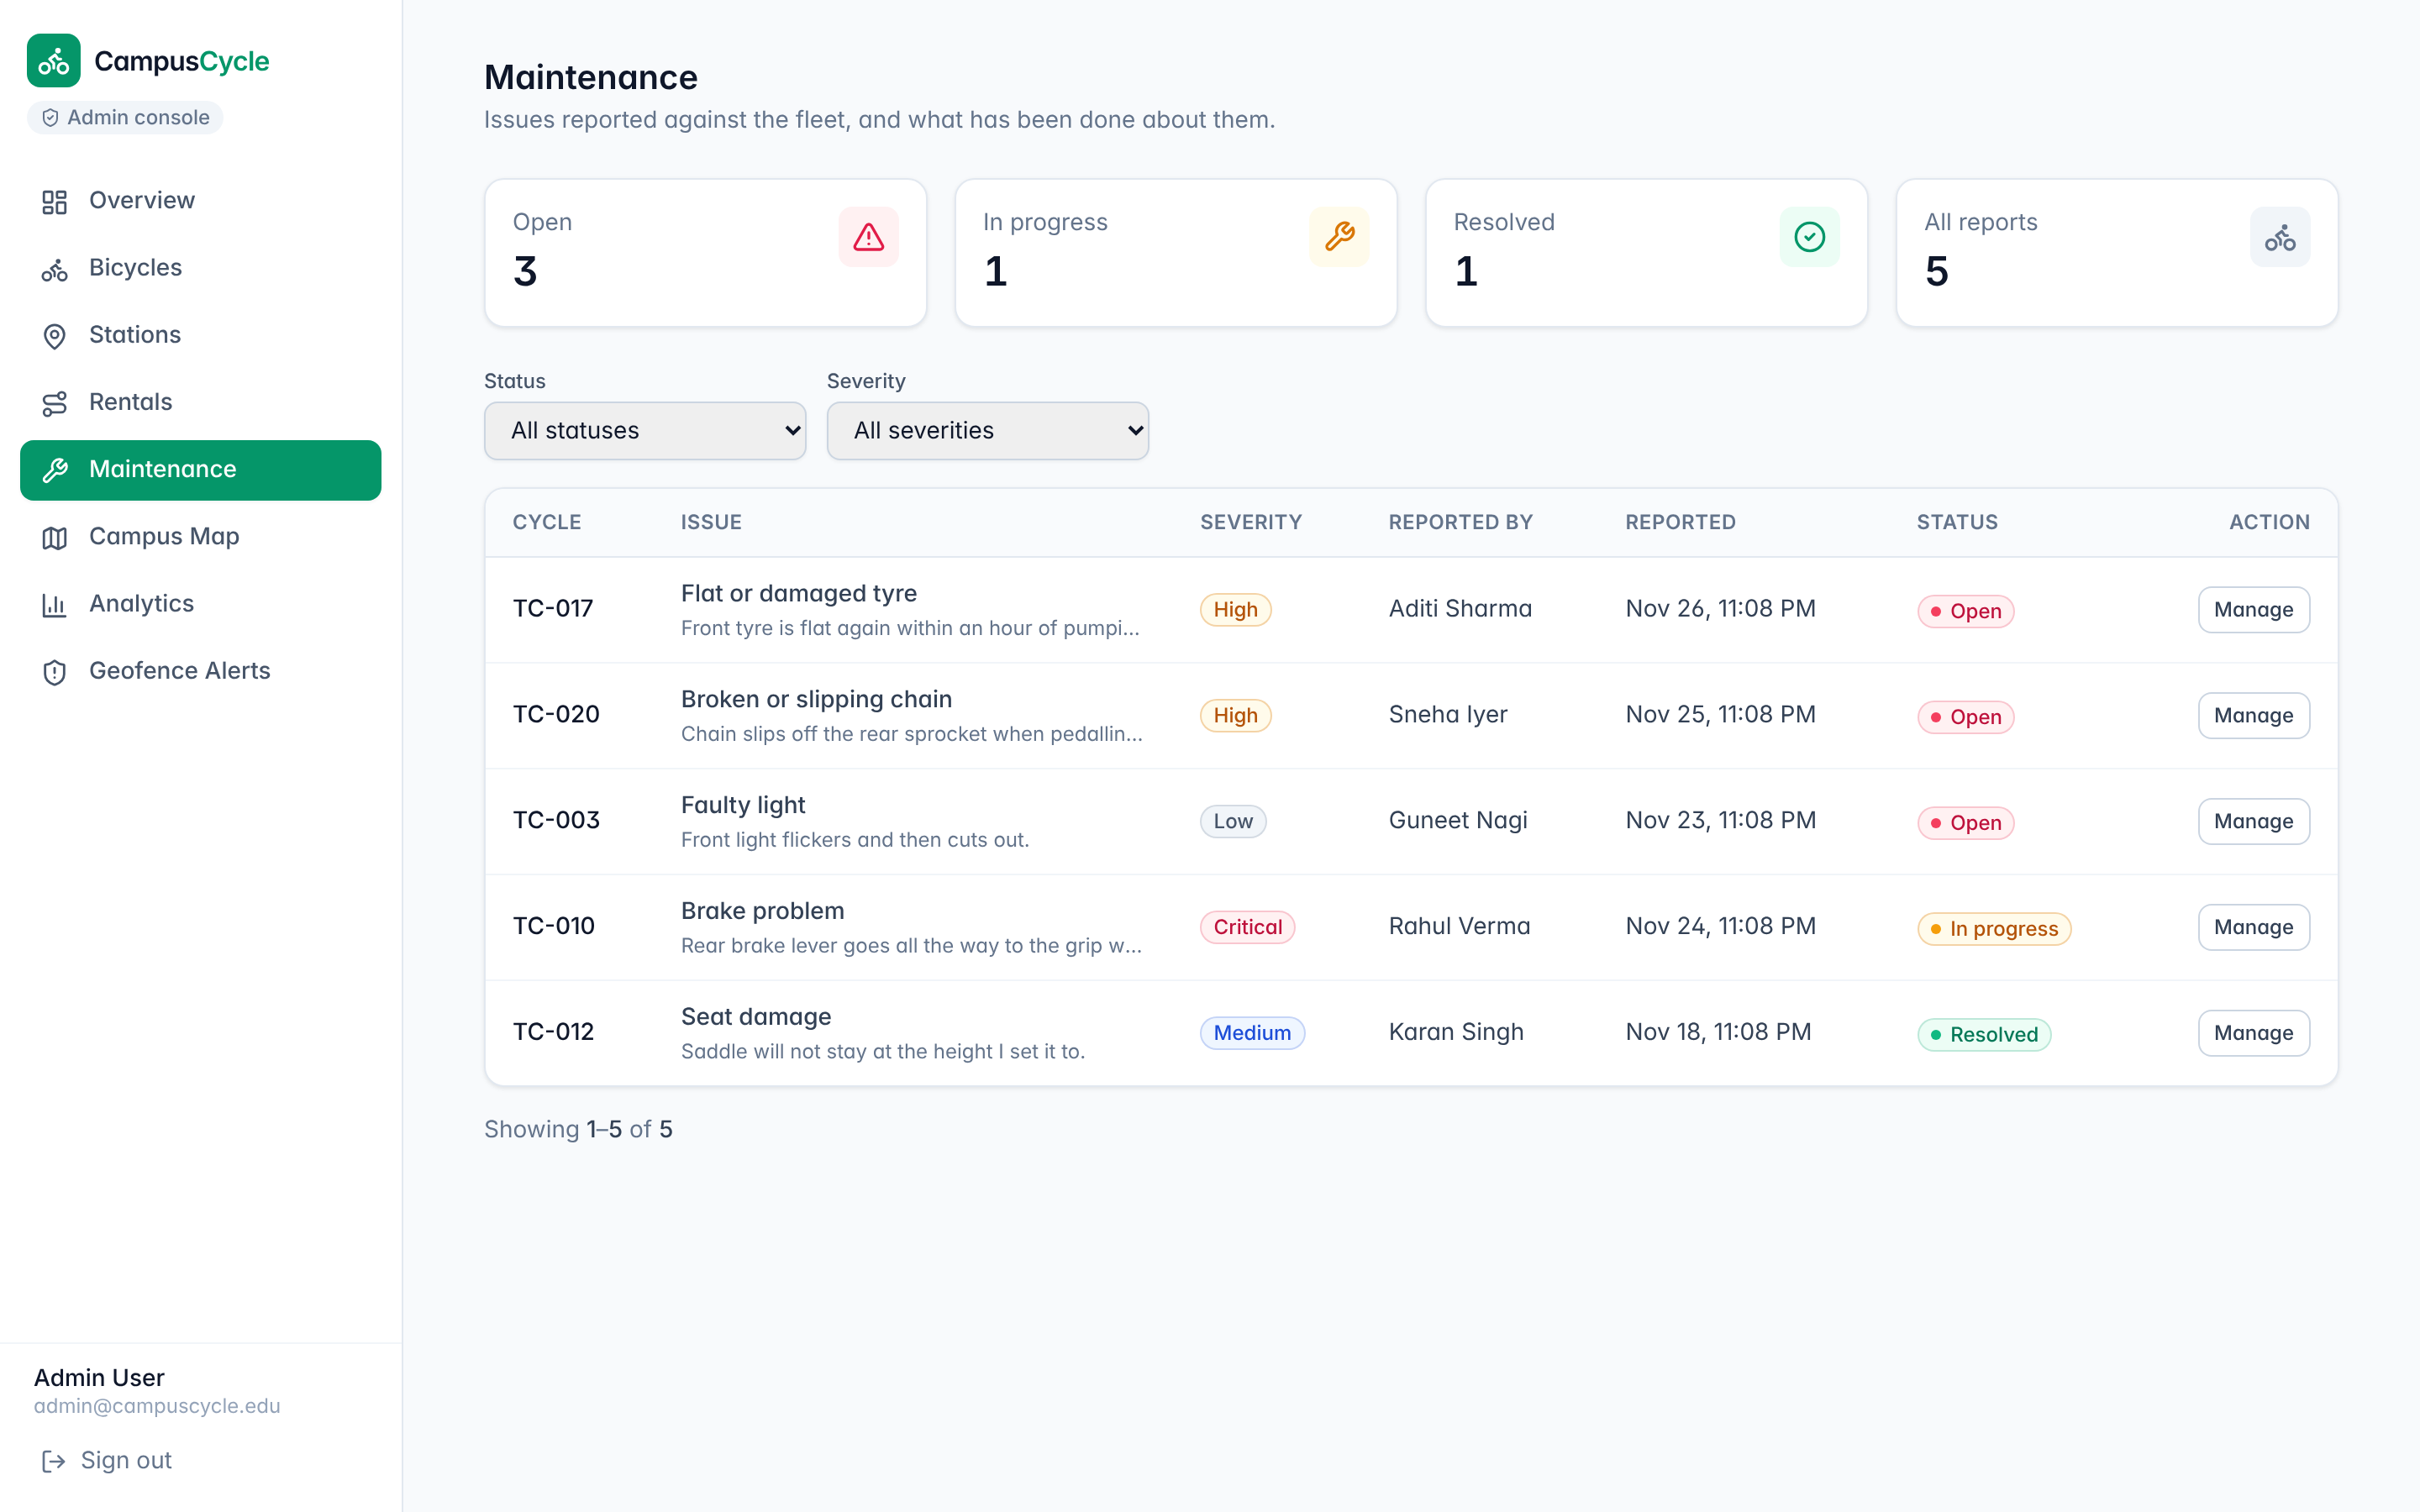
\includegraphics[width=\textwidth]{figures/ui-admin-maintenance.png}
  \caption{Administrative maintenance queue. Only the
    transitions permitted from a report's current
    state are offered.}
  \label{fig:uimaint}
\end{figure}

\subsection{Usage Analytics}
\label{sec:analytics}

Every figure on the analytics dashboard
(Figures~\ref{fig:uianalytics} and~\ref{fig:uicharts})
is a PostgreSQL aggregate over the live tables;
nothing is cached or hard-coded. The page separates
two kinds of number that are easily confused: a
\emph{snapshot} of the fleet together with all-time
totals, which the date filter does not affect, and
\emph{period} figures counting only rides that started
inside the selected range. The two groups are given
separate headings on screen for that reason.

Three details were necessary for the figures to be
trustworthy. Empty days are generated with
\texttt{generate\_series} and joined against, so a
quiet week produces zeros on a continuous axis rather
than a gap. Averages over an empty set return no value
rather than zero, which are different statements. Day
and hour buckets are computed in an explicitly
configured reporting timezone, because
\texttt{date\_trunc} otherwise follows the database
session's timezone: during development this placed
rides on the wrong calendar day whenever the server
session ran in UTC while the campus is at
UTC$+$05:30.

\begin{figure}[htbp]
  \centering
  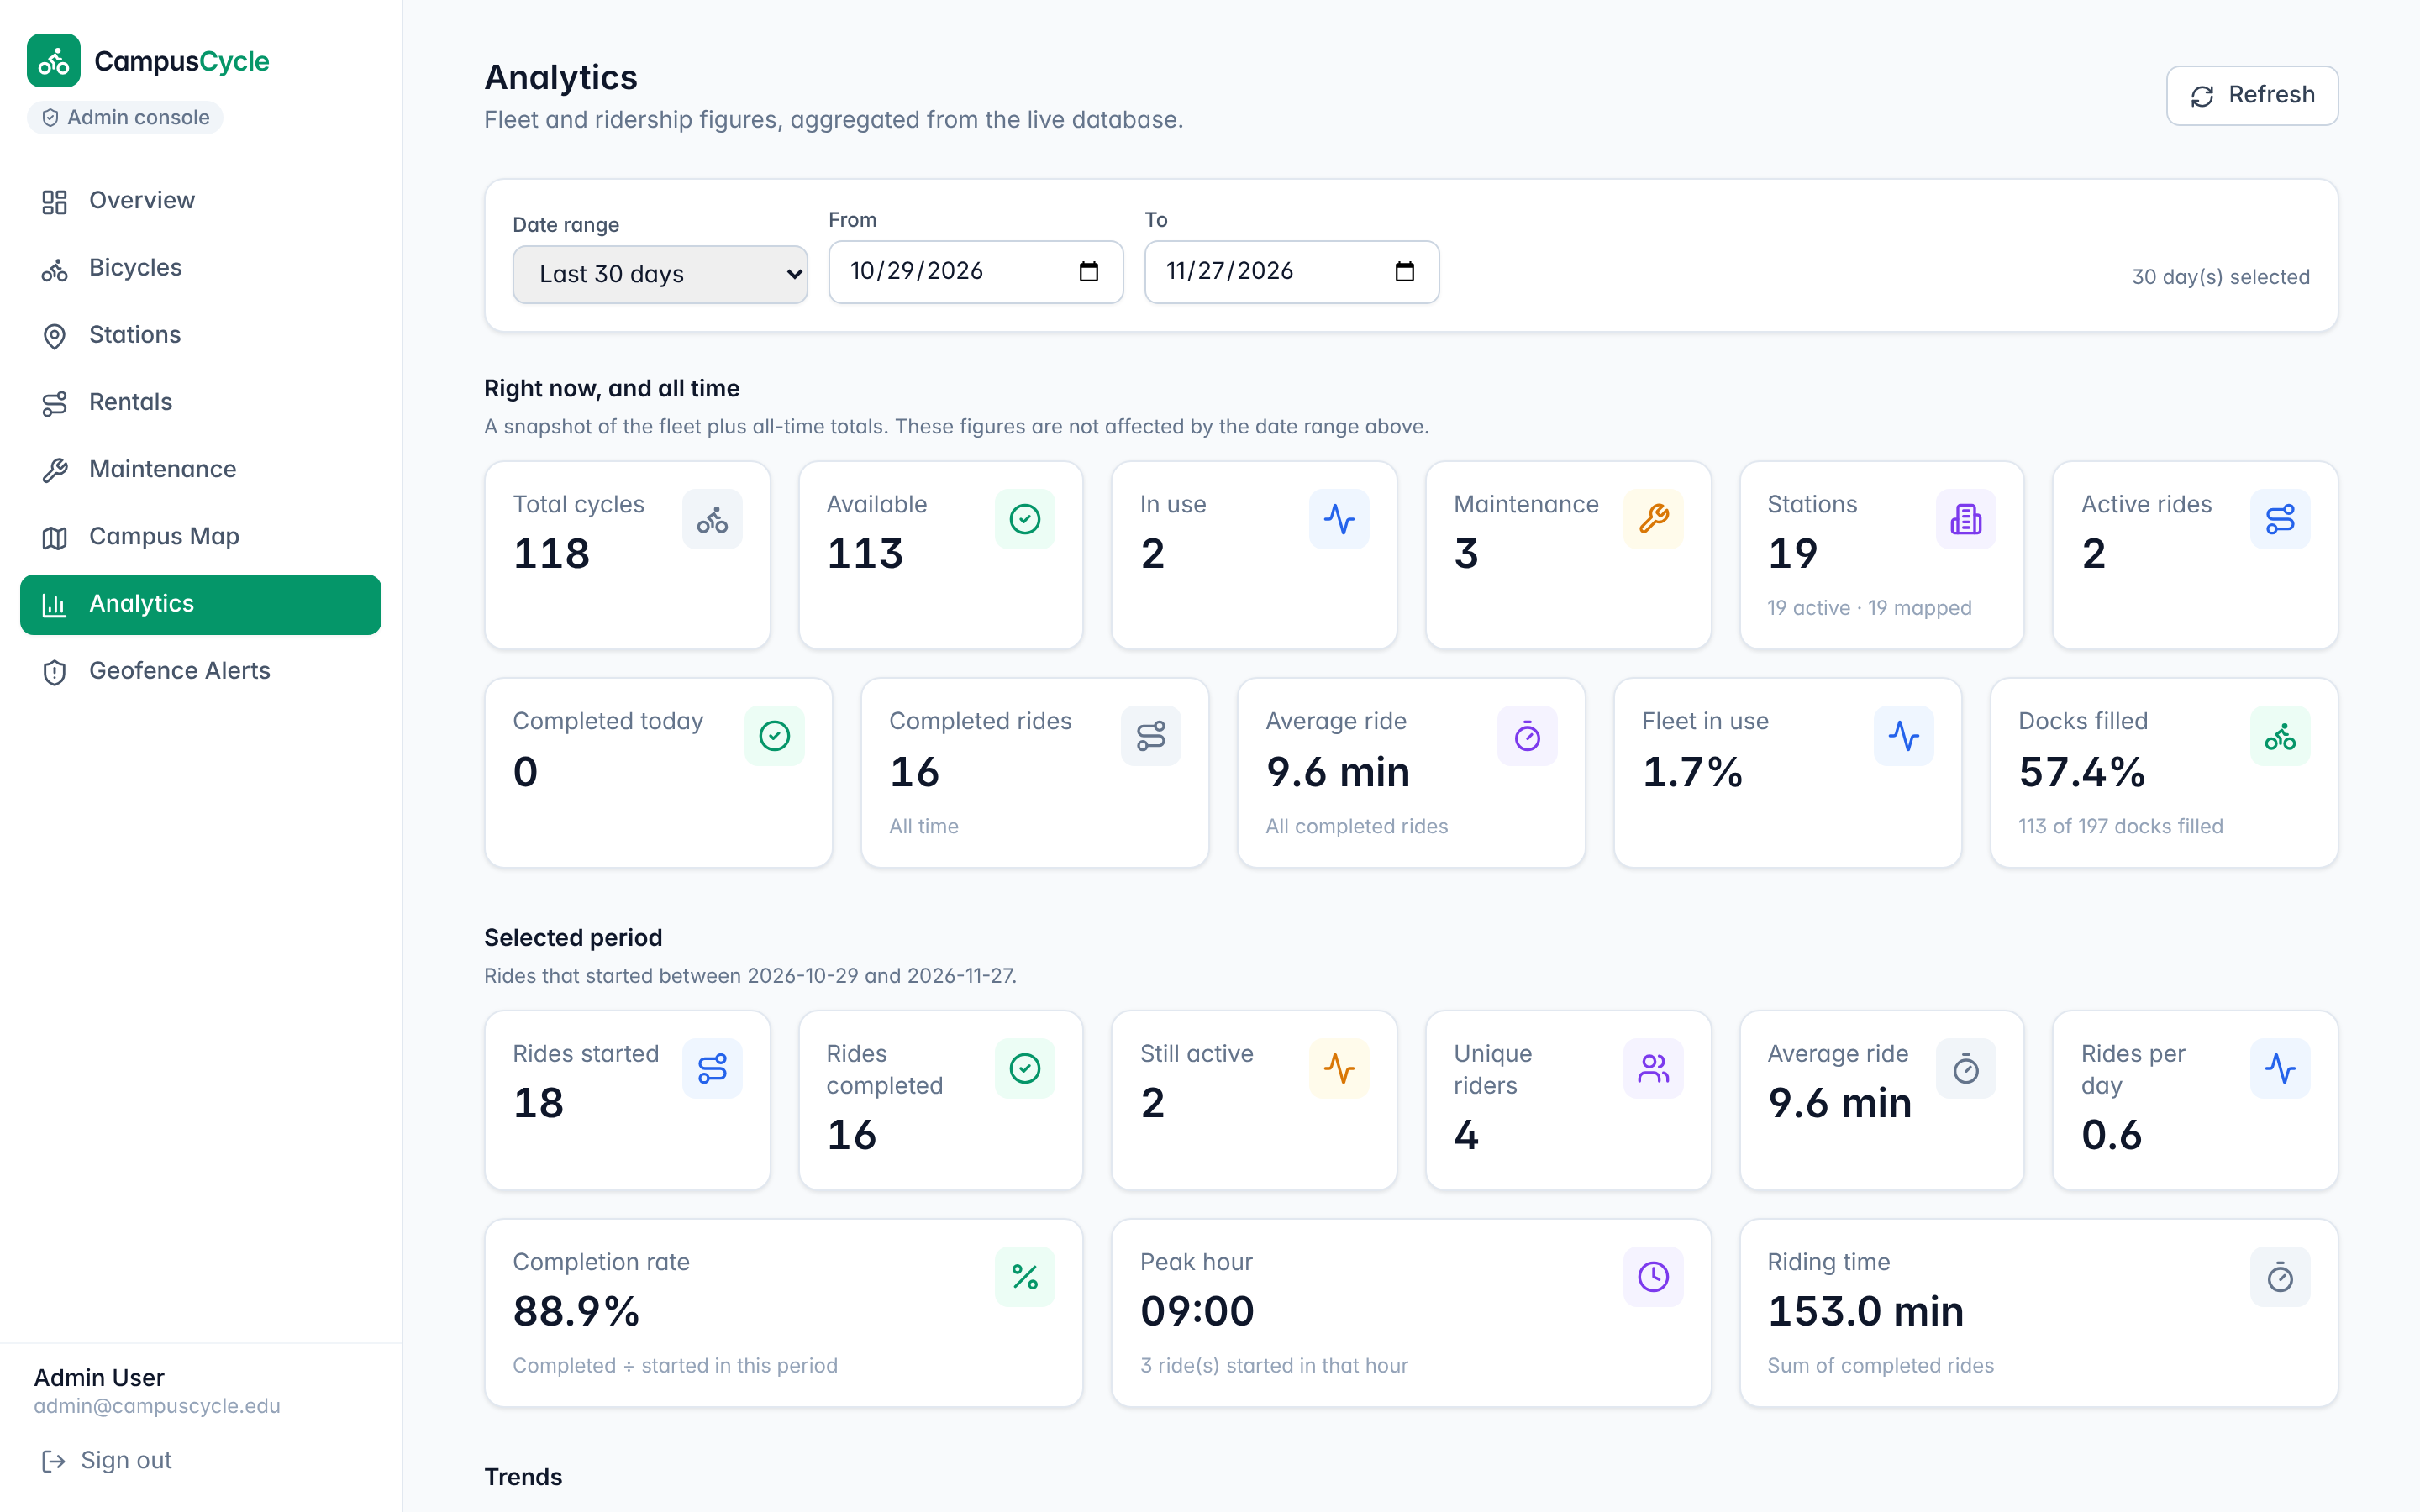
\includegraphics[width=\textwidth]{figures/ui-admin-analytics.png}
  \caption{Analytics dashboard. Snapshot and all-time
    figures are kept visually and textually separate
    from figures for the selected period.}
  \label{fig:uianalytics}
\end{figure}

\begin{figure}[htbp]
  \centering
  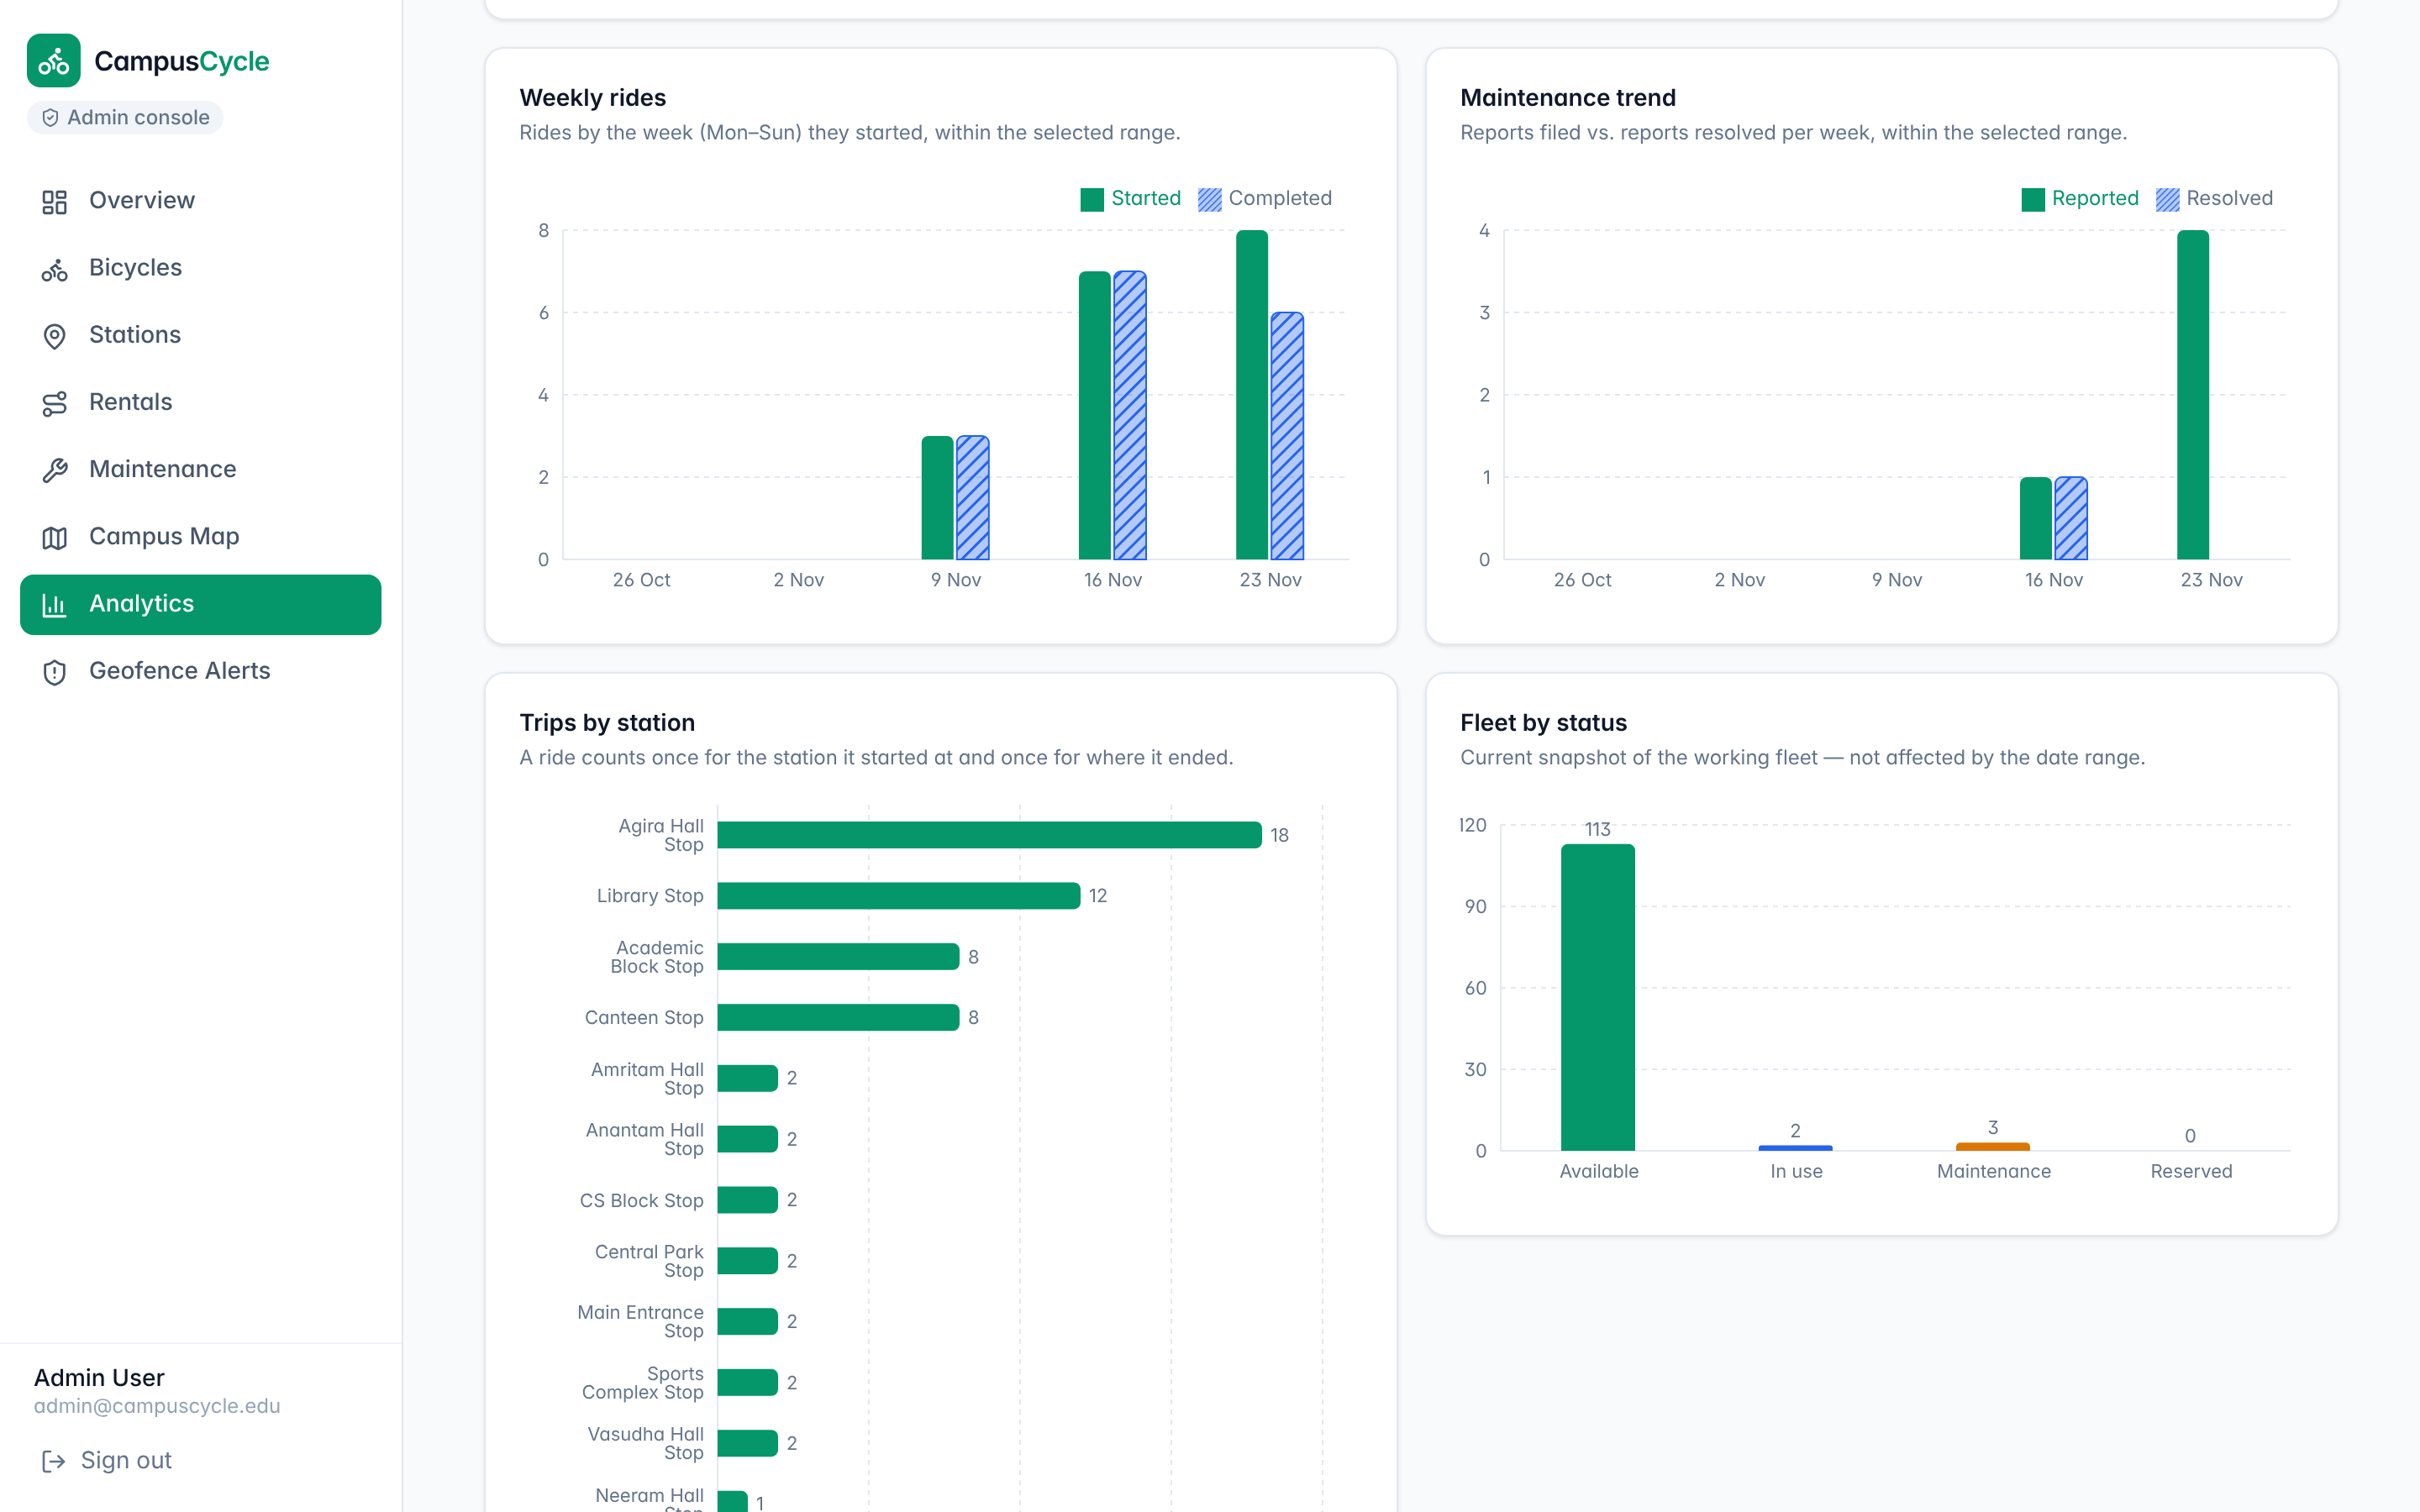
\includegraphics[width=\textwidth]{figures/ui-admin-analytics-charts.png}
  \caption{Trends and distributions on the same page,
    each drawn from its own aggregate query.}
  \label{fig:uicharts}
\end{figure}

\subsection{Software-Based Geofencing}
\label{sec:geofence}

\textbf{The bicycles carry no GPS hardware.} There is
no continuous tracking in this system, and the
application does not present one. Every position it
holds was explicitly submitted through an
administrator-only endpoint and is stored with its
source; only simulated positions are accepted, and a
position claiming to come from a device is rejected
until a real integration exists. A student's browser
location is never accepted as a bicycle's position,
which is why the endpoint takes an explicit cycle
identifier and is closed to students.

The campus boundary is a configurable polygon stored
as JSONB and tested with a ray-casting
point-in-polygon algorithm~\cite{shamos1976}; at the
scale of one campus, treating latitude and longitude
as a plane introduces no meaningful error. A position
outside the boundary opens an alert recording the
cycle, the time, the coordinates and the ride in
progress. A \emph{repeated} breach does not open
another: it increments the existing alert's counter
and updates its last known position, a rule enforced
by the partial unique index named earlier. A cycle
seen back inside records that fact but does not close
the alert, because whether the situation is resolved
is a judgement for a person. In
Figure~\ref{fig:uigeofence} the cycle \texttt{TC-004}
was reported outside the boundary three times and
appears once, with an update count of three.

\begin{figure}[htbp]
  \centering
  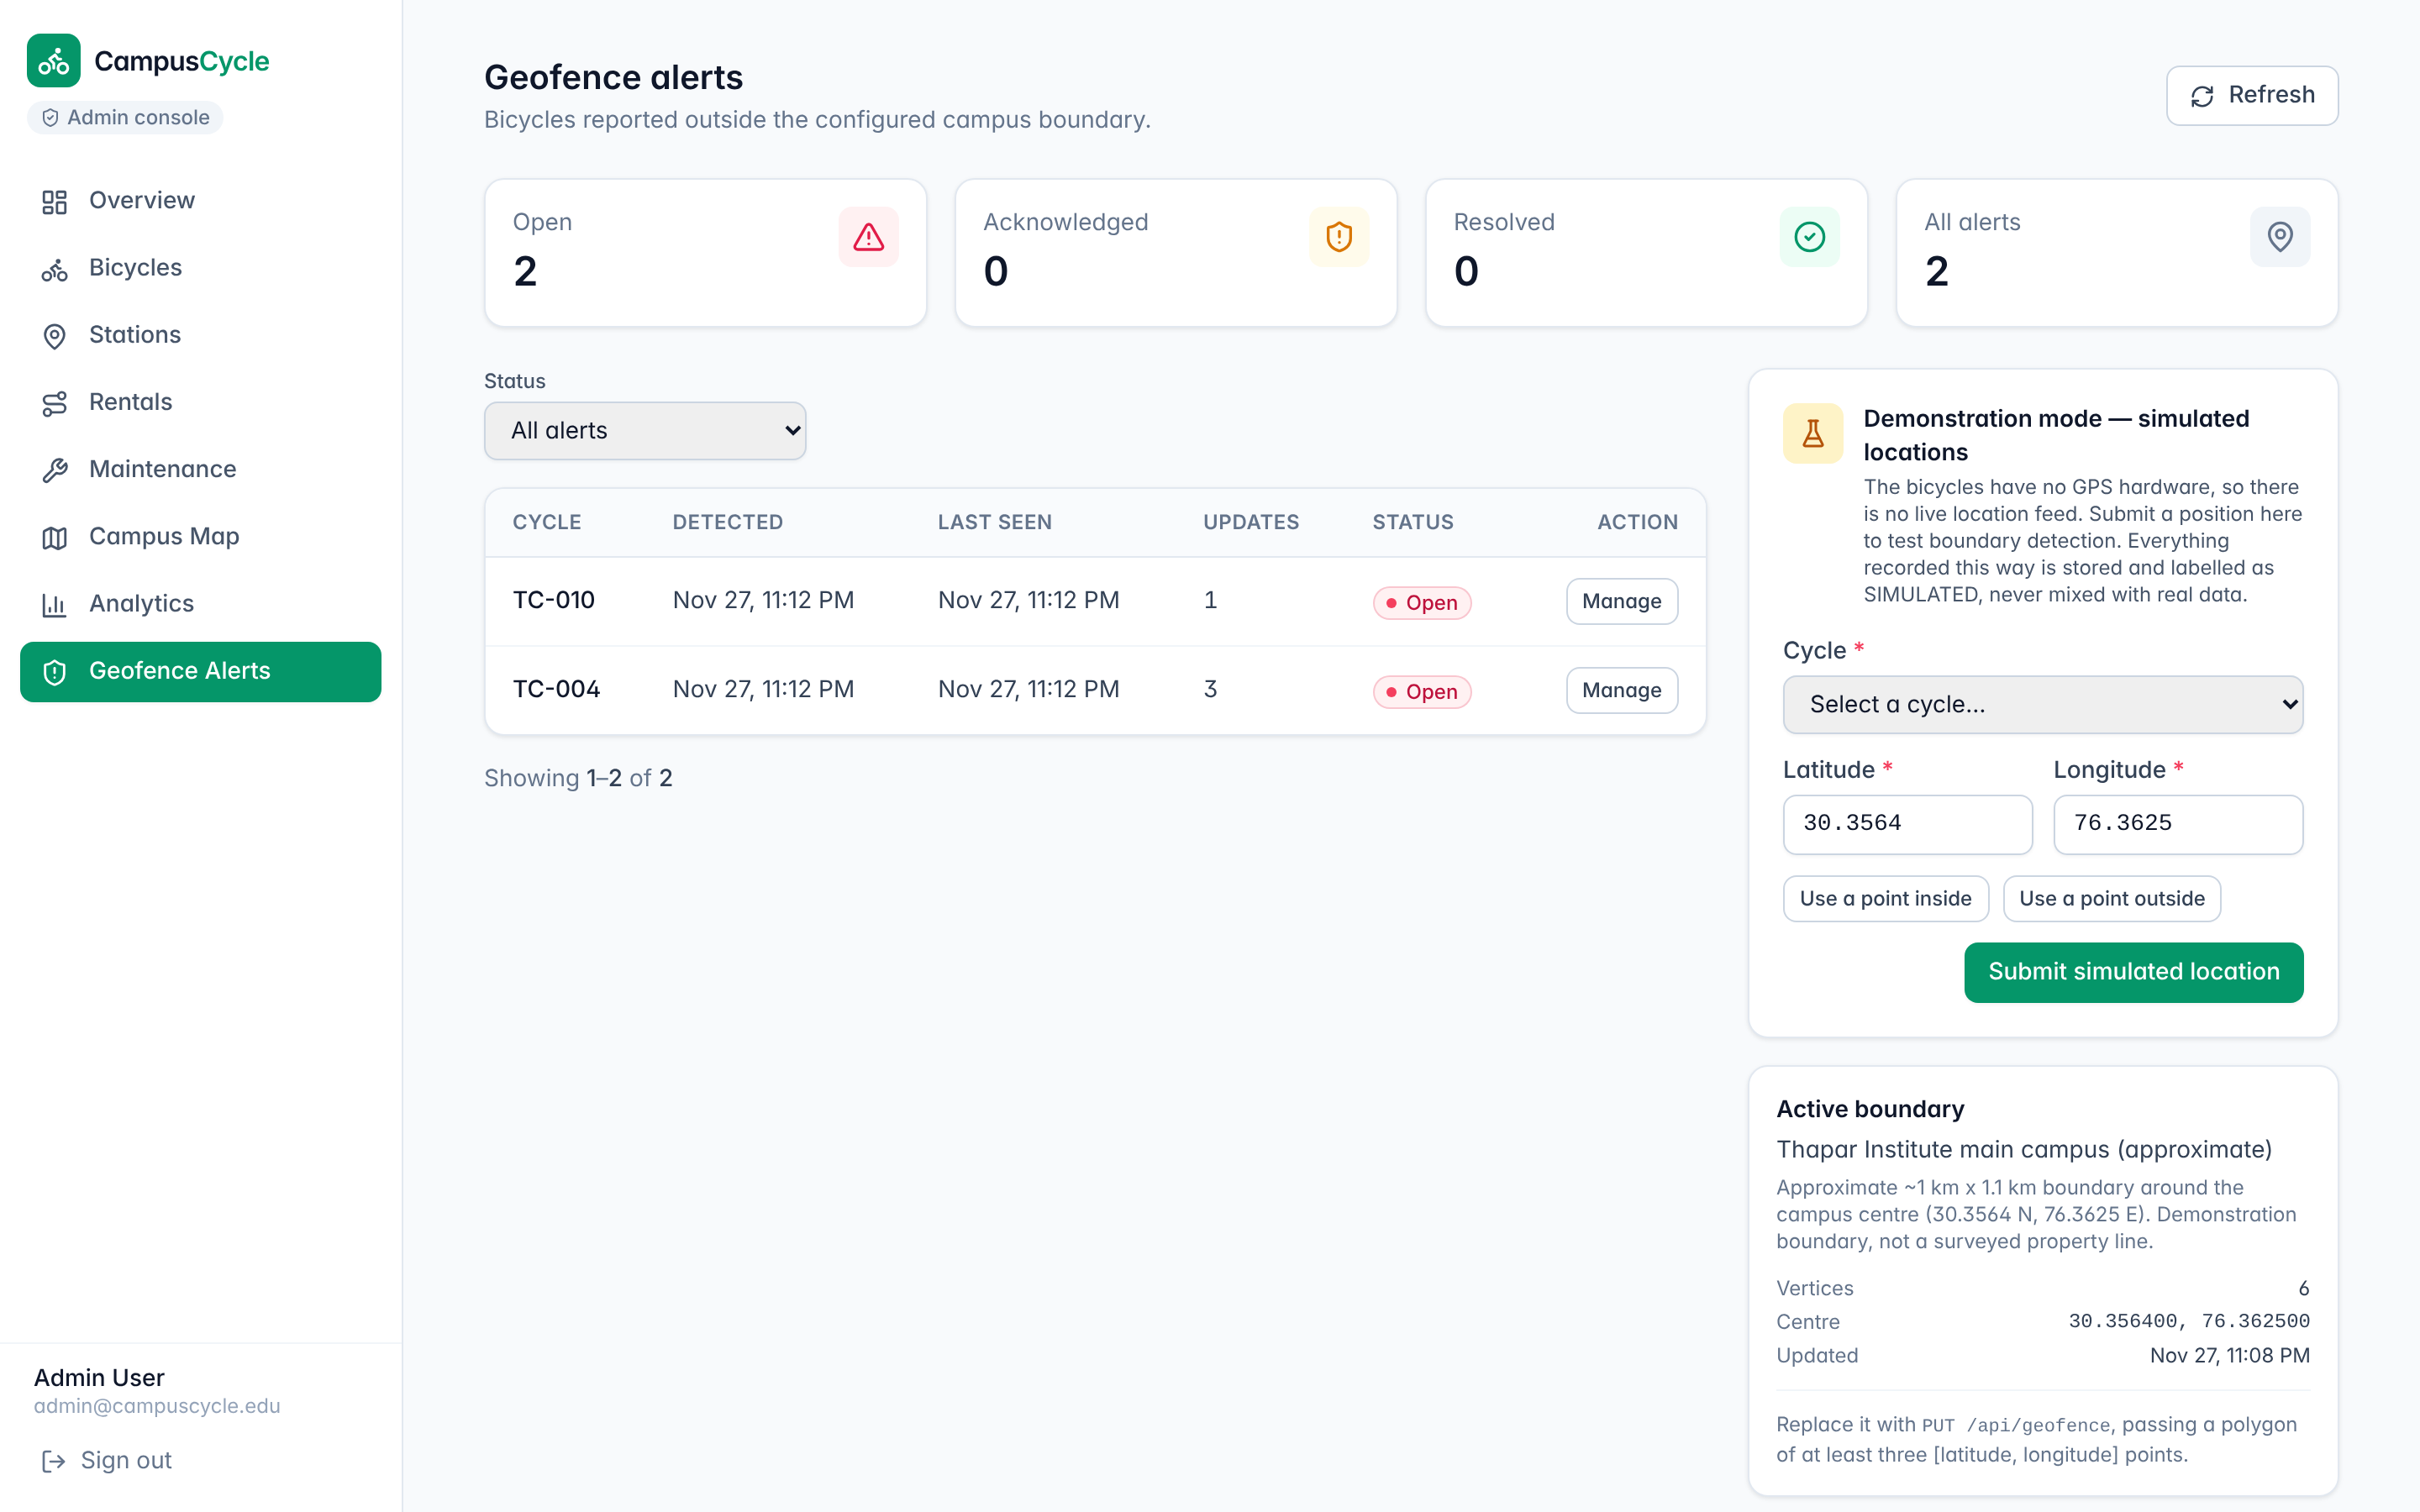
\includegraphics[width=\textwidth]{figures/ui-admin-geofence.png}
  \caption{Geofence alerts. Three breaches of
    \texttt{TC-004} produced one alert with three
    updates, not three alerts. The demonstration panel
    that submits simulated positions is labelled as
    such on screen.}
  \label{fig:uigeofence}
\end{figure}

\section{Security Considerations}

\begin{itemize}
  \item \textbf{Credentials.} Passwords are stored
    only as bcrypt hashes. Sign-in failures return one
    uniform message, so the response cannot be used to
    discover which email addresses are registered.
  \item \textbf{Authorisation.} Role checks sit in
    middleware on the route, not in the handler, so an
    endpoint cannot be added without a decision about
    who may reach it.
  \item \textbf{Injection.} Every query is
    parameterised; no SQL is assembled from user
    input.
  \item \textbf{Secrets.} The JWT secret and database
    credentials are read from the environment, and the
    environment file is excluded from version control.
    A test asserts that no password hash, token secret
    or connection string appears in any API response.
  \item \textbf{Transport and headers.} \texttt{helmet}
    sets standard security headers, CORS is restricted
    to the configured origin, and authentication
    endpoints are rate limited.
\end{itemize}

% ===== CHAPTER 3: RESULTS & EVALUATION =====

\chapter{Results and Evaluation}

\section{Testing Methodology}

Testing is automated and runs against a real
PostgreSQL database rather than a mocked one, because
most of the properties worth testing in this system
--- uniqueness under concurrency, transactional
consistency, the correctness of aggregate queries ---
exist only in the database and would be assumed away
by a mock. The suites refuse to run against any
database whose name does not end in \texttt{\_test},
since they rebuild the schema before each run.

\begin{itemize}
  \item \textbf{Integration and end-to-end testing.}
    Three suites rebuild the schema, apply the
    migrations, load the seed data, start the Express
    application on an ephemeral port and drive it over
    real HTTP. They cover the full rental lifecycle,
    role-based access control, the maintenance and
    safety-hold workflow, analytics figures checked
    against direct SQL counts, geofence detection and
    de-duplication, and the campus map and routing
    endpoints.
  \item \textbf{Unit testing.} The route planner is
    tested without a database, directly against the
    traced road network: that every stop sits on a
    road, that a route exists between all 342 ordered
    pairs of the 19 stops, that no route is shorter
    than the straight-line distance, and that specific
    routes follow the roads a reader can check by eye
    on the map.
  \item \textbf{Concurrency testing.} Two sign-ins
    issue simultaneous requests for the same bicycle;
    the suite asserts that exactly one succeeds and
    one is refused.
  \item \textbf{Regression testing.} Each earlier
    phase's suite is run unchanged after every later
    change. The only modification across three phases
    was to apply new migrations before seeding; no
    assertion was altered or removed.
  \item \textbf{Empty-database testing.} A dedicated
    group of checks runs every read endpoint against a
    database with no rows at all, asserting that the
    analytics page returns zeros and nulls rather than
    \texttt{NaN}, and that no page fails.
  \item \textbf{User-interface testing.} Two browser
    suites drive the real interface end to end: a
    student files a critical fault report and the
    cycle disappears from the rentable list, an
    administrator resolves it and is offered the
    return-to-service action, and the campus map
    renders markers and plans a route between two
    stops.
  \item \textbf{Build verification.} The production
    frontend build is run as part of the check, so a
    broken import or unused dependency fails
    immediately.
\end{itemize}

\section{Results}

The four automated suites below were re-run from a
clean PostgreSQL~16 database while this report was
being prepared. All checks pass
(Table~\ref{tab:tests}).

\begin{table}[htbp]
\centering
\begin{tabular}{@{}lrrl@{}}
\toprule
\textbf{Suite} & \textbf{Checks} & \textbf{Passed} &
\textbf{Covers} \\
\midrule
Route planner (unit)  & 14  & 14  & Road graph, stop
  snapping, \\
                      &     &     & shortest paths \\
Phase~1 end-to-end    & 26  & 26  & Rental lifecycle,
  RBAC, concurrency \\
Phase~2 end-to-end    & 145 & 145 & History,
  maintenance, analytics, \\
                      &     &     & geofencing, access
  control \\
Phase~3 end-to-end    & 100 & 100 & Campus map, routing,
  availability, \\
                      &     &     & empty-database
  behaviour \\
\midrule
\textbf{Total}        & \textbf{285} & \textbf{285} & \\
\bottomrule
\end{tabular}
\caption{Automated test results. All suites pass with
  no failures.}
\label{tab:tests}
\end{table}

A selection of the properties asserted, chosen because
each corresponds to an objective rather than to a
screen:

\begin{itemize}
  \item Two students requesting the same bicycle
    simultaneously produce exactly one rental and one
    refusal.
  \item A seeded 38-minute ride reports a duration of
    exactly 2280 seconds; a ride still in progress
    reports a duration that advances.
  \item A student requesting another student's ride
    receives 403; an unknown ride identifier receives
    404; a malformed one receives 400.
  \item A cycle with an unresolved critical report
    cannot be rented, and an administrator attempting
    to mark it available receives 409.
  \item Three successive out-of-bounds positions
    produce one alert with a count of three, not three
    alerts.
  \item A route exists between all 342 ordered pairs
    of stops, and every stop lies within six pixels of
    a mapped road.
  \item Against an empty database, the analytics
    endpoints return zeros and nulls and never
    \texttt{NaN}.
  \item Every administrative endpoint returns 403 for
    a student token and 401 for no token.
  \item No password hash, token secret or connection
    string appears in any API response.
\end{itemize}

\section{Scale of the Implementation}

\begin{table}[htbp]
\centering
\begin{tabular}{@{}lr@{}}
\toprule
\textbf{Measure} & \textbf{Value} \\
\midrule
Backend source files            & 62 \\
Backend lines of code           & 7{,}129 \\
Frontend source files           & 69 \\
Frontend lines of code          & 9{,}486 \\
SQL (schema, migrations, seeds) & 866 \\
REST endpoints                  & 47 \\
Database tables                 & 8 \\
Indexes and unique constraints  & 24 \\
Campus stops mapped             & 19 \\
Automated checks                & 285 \\
\bottomrule
\end{tabular}
\caption{Implementation size at this evaluation.}
\label{tab:size}
\end{table}

\section{Analysis}

\subsection{Were the Objectives Met?}

Eight of the nine objectives are complete and
evidenced by the tests listed above. The ninth, demand
prediction, was not implemented, for the reason given
in Section~\ref{sec:scope}.

One completed objective deserves a qualified answer.
The geofencing objective is met as specified --- a
boundary is configurable, violations are detected,
recorded, de-duplicated and actionable --- but it
operates on submitted positions rather than measured
ones, because the project has no GPS hardware. Rather
than let the interface imply a tracking capability
that does not exist, the limitation is made explicit
in the API, in the stored data and on screen. The
software is structured so that the eventual hardware
feed replaces one validated input path and nothing
else.

\subsection{Challenges and Their Resolution}

\paragraph{Concurrent access to a single bicycle.}
The first implementation checked a bicycle's
availability and then created the rental, which is
correct when tested by one person and wrong under
load: two requests can both pass the check before
either writes. The resolution was to stop treating
this as application logic. The bicycle row is locked
for the duration of the transaction, and a partial
unique index makes a second active rental impossible
even if the lock were somehow bypassed. The
concurrency test exists to prove the fix rather than
to illustrate the feature.

\paragraph{Keeping a safety rule true everywhere.}
A bicycle can become available through three
different paths: an administrator sets its status, a
ride ends, or it is created. An early version checked
for unresolved faults only in the first. The
resolution was to make the safety hold a single
function consulted by all three paths, and to express
it as a property of the maintenance records rather
than as an extra column on the bicycle --- a flag
would have been one more piece of state capable of
disagreeing with the reports it summarises.

\paragraph{Timezone-dependent analytics.} Rides were
being attributed to the wrong calendar day. The cause
was that day boundaries were computed in Node using
the machine's local timezone while PostgreSQL grouped
them using the database session's timezone. The
resolution was to make the reporting timezone an
explicit configuration value used on both sides, so
that ``today'' means one thing throughout the system.

\paragraph{Routes that cut through buildings.} The
first version of the campus map drew a straight line
between two stops, which is useless advice on a campus
where the direct line crosses a cricket field and two
hostels. The resolution was to trace the roads drawn
on the map into a graph and run a shortest-path search
over it, so that a route is a sequence of real roads.
The unit suite was written first and includes a check
that a specific pair of stops is routed around a field
rather than across it.

\paragraph{Two coordinate systems at once.} Phase~3
needed positions on an illustration while Phase~2's
geofencing needed real latitude and longitude. The
temptation was to georeference the artwork and keep
one system. The resolution was the opposite: keep both
and never mix them. The map columns are percentages of
an image, the geofence columns are degrees, each is
range-checked separately, and no code converts between
them --- because any such conversion would be a
fiction about an illustration that was never surveyed.

\paragraph{Migrating a database already in use.} The
schema had to change twice without discarding earlier
data. The resolution was to separate the destructive
development path from the additive production path:
the base schema remains re-runnable for a fresh
install, while each migration adds only what is
missing and can be run repeatedly without effect.

% ===== CHAPTER 4: CONCLUSION =====

\chapter{Conclusion}

\section{Summary of Work}

CampusCycle is a working campus bicycle-sharing
system. Students sign in, find an available cycle on
an illustrated map of their own campus, plan a route
to it along the roads that exist, identify the cycle
by its QR code, ride it between stops, return it,
review their ride history and report faults.
Administrators manage stops and the fleet, inspect
every ride, work reported faults through a maintenance
lifecycle, read usage analytics computed from the live
database and act on geofence alerts.

Across three phases the system comprises 47 REST
endpoints over eight PostgreSQL tables, with 285
automated checks passing against a real database. Each
phase was delivered without modifying a single
assertion from an earlier one and without rebuilding
the database it inherited.

\section{Key Findings}

\begin{itemize}
  \item \textbf{Invariants belong in the database.}
    Every rule that had to survive concurrent use ---
    one active ride per student, one per cycle, one
    unresolved alert per bicycle --- is enforced by a
    partial unique index. Application code states the
    rule clearly and produces a readable error; the
    database guarantees it.

  \item \textbf{A rule enforced in one place is a rule;
    enforced in three, it is a coincidence.} The
    safety hold became reliable only once every path
    that could make a bicycle available consulted the
    same check. The same applies to availability: one
    definition is why the map and the stop list cannot
    disagree.

  \item \textbf{Authorisation must not be derived from
    the request.} Taking the user's identity from the
    verified token rather than from a request
    parameter makes ``a student sees only their own
    rides'' a property of the system rather than a
    property of each endpoint.

  \item \textbf{An honest limitation is cheaper than a
    convincing one.} Labelling simulated positions as
    simulated, reporting map distances as approximate
    and estimating no travel time at all cost a column
    and a few validation rules. It leaves the system
    extensible to real hardware and prevents an
    operator from ever mistaking a demonstration for
    evidence.

  \item \textbf{A diagram is a design tool, not an
    illustration.} Redrawing the data-flow diagrams at
    the level of individual checks, with invariant
    flows marked, surfaced the deferred-hold path in
    Figure~\ref{fig:dfd2r} as a distinct process
    rather than an implementation detail --- which is
    where it belongs, because forgetting it would
    return an unsafe cycle to service.
\end{itemize}

\section{Limitations}

\begin{itemize}
  \item There is no real-time tracking; bicycle
    positions are administrator-submitted and
    simulated.
  \item There is no demand prediction or
    redistribution advice.
  \item Rides are free. No pricing, wallet or payment
    integration exists.
  \item The campus map is an illustration, not a
    survey. Route distances are approximate and no
    travel time is estimated.
  \item The geofence boundary approximates the campus
    extent rather than the legal property line.
  \item There is no password-reset or email
    verification flow.
  \item The system has run in demonstration use rather
    than campus-wide service, so the recorded
    ridership history is small.
\end{itemize}

\section{Future Work and Recommendations}
\label{sec:futurework}

\begin{enumerate}
  \item \textbf{Demand prediction.} Train a regression
    or tree-based model on recorded rental history
    using stop, hour of day, day of week and recent
    demand as features. The analytics layer already
    produces these aggregates, so the model would
    consume a stable schema rather than ad-hoc
    extraction. This requires a term of real ridership
    data first.

  \item \textbf{Redistribution advice.} Compare
    predicted demand against current stop occupancy
    and recommend movements. This requires no new
    data, only the model from the previous item.

  \item \textbf{GPS and IoT integration.} Fit tracking
    units and allow device-sourced positions. The
    ingestion path, the storage, the boundary test and
    the alerting already exist; the change is to admit
    a second value in the source column and to accept
    authenticated device traffic.

  \item \textbf{Electronic locks.} With trusted
    hardware the QR workflow could unlock a physical
    lock, closing the gap between a rental record and
    physical possession of the cycle.

  \item \textbf{Payments and membership.} Semester
    passes, penalties for late returns and receipts,
    should the service move beyond free use.

  \item \textbf{Deployment hardening.} Refresh tokens
    with rotation, structured logging, automated
    backups and a continuous integration pipeline
    running the existing suites on every push.
\end{enumerate}

\section{Final Remarks}

The most useful lesson from this project was about
where correctness lives. The features that were
straightforward to build were the ones that are
visible: a form, a list, a chart. The ones that took
real design effort were invisible when working and
only noticeable when broken --- two students must not
get the same bicycle, a cycle reported unsafe must not
reappear as available, a student must not see another
student's rides. Each of these was first written as
application logic, and each became reliable only once
it was pushed down to a single enforcement point,
usually a database constraint, with the application
code reduced to stating the rule clearly and
explaining the refusal.

The second lesson concerns honesty in engineering. It
would have been easy to present the geofencing module
as bicycle tracking, or to put a confident number of
minutes next to a route measured off a drawing. The
screens would have looked better. Recording the
provenance of every position, labelling map distances
as approximate and declining to estimate travel times
cost very little and leaves both the system and its
documentation truthful about what has actually been
built --- which is also what makes the hardware phase
a straightforward extension rather than a correction.

% ===== BIBLIOGRAPHY =====

% Print bibliography with heading in TOC
\printbibliography[heading=bibintoc]

\end{document}
